%\linebreak
\documentclass[a4paper,12pt]{report}
\usepackage[utf8x]{inputenc}
\usepackage[usenames,dvipsnames,svgnames,table]{xcolor}
\usepackage{fancyvrb}
\usepackage{float}
\usepackage{booktabs}
\usepackage{multirow}


\usepackage[round]{natbib}
\bibliographystyle{dinat}
\usepackage{alltt}
\usepackage{adjustbox}
\usepackage[usenames,dvipsnames,svgnames,table]{xcolor}
\usepackage[T1]{fontenc}
\usepackage[francais]{babel}
\usepackage{url} % Pour écrire des adresses cliquables.
\usepackage{lmodern} % Pour changer le pack de police.
\usepackage[top=2.5cm, bottom=2.5cm, left=2.5cm, right=2.5cm]{geometry}
\usepackage{fancyhdr}
\usepackage{graphics}
\usepackage{graphicx}
\usepackage{color}
\usepackage{colortbl}
\usepackage{url}
\usepackage{amsfonts}
\usepackage{amsmath}
\usepackage[french]{minitoc}
\usepackage[colorlinks]{hyperref}
\usepackage[gen]{eurosym}
\usepackage{caption}
\usepackage[nottoc, notlof, notlot]{tocbibind}
\usepackage{pdfpages}
\usepackage[Lenny]{fncychap}
\usepackage{fancyhdr}
\usepackage{amsmath}
\usepackage{epigraph}
\usepackage{setspace}
\linespread{1.5}
\usepackage{booktabs}
\usepackage{makecell}
\usepackage{tabularx}


 
 
\hypersetup{	
colorlinks=true, %colorise les liens 
breaklinks=true, %permet le retour à la ligne dans les liens trop longs 
urlcolor= blue, %couleur des hyperliens 
linkcolor= blue,	%couleur des liens internes 
citecolor=blue,	%couleur des références 
pdftitle={}, %informations apparaissant dans 
pdfauthor={}, %les informations du document 
pdfsubject={},	%sous Acrobat. 
pdfcreator={}
}


\pagestyle{fancy}
\setcounter{page}{1}
\fancyhead[L]{\leftmark}
\fancyhead[R]{}

\fancyfoot[C]{}
\fancyfoot[R]{\thepage}
%%%%%%%%%%%%%%%%%%%%%%%%%%%%%

%%%%%%%%%%%%%%%%%%%%%%%%%%%%%

\newtheorem{thrm}{Théorème}
\newtheorem{prop}{Proposition}
\newtheorem{defin}{Définition}
\newtheorem{algo}{Algorithme}
\newtheorem{exmpl}{Exemple}
\newtheorem{res}{Résultat}
%\newcommand{\pchapter}[2]{
 %   \setcounter{chapter}{#1}
  %  \setcounter{section}{0}
   % \chapter*{#2}
%}
\setcounter{tocdepth}{3}% Include \subsubsection in ToC
\setcounter{secnumdepth}{4}% Number \subsubsection

\newcommand{\intervalleoo}[2]{\mathopen{]}#1\,;#2\mathclose{[}}
\newcommand{\intervalleff}[2]{\mathopen{[}#1\,;#2\mathclose{]}}
\newcommand{\intervalleof}[2]{\mathopen{]}#1\,;#2\mathclose{]}}
\newcommand{\intervallefo}[2]{\mathopen{[}#1\,;#2\mathclose{[}}
\newcommand{\intervalle}[2]{\mathopen{(}#1\,;#2\mathclose{)}} 


\begin{document}
\pagenumbering{roman}	

	\newpage
		\begin{center}
			
\includegraphics[width=0.5\linewidth]{./images/u-paris10.png}
			\vspace{1cm}
		\end{center}
			
		\begin{center}
			\vspace{0.3cm}
			\large  
			\textbf{Mémoire Master 2 MIAGE classique}\\
			\vspace{0.7cm} \large Thème\\
			\vskip 0.2in
		\end{center}
		

		\begin{center}
        	\hrule
        \vspace{.7cm}
        {\Huge\textbf{ Etude des approches de modélisation des entrepôts de données (DataWarehouse)}}\\
        \vspace{.7cm}
            \hrule
		\end{center}			
		
			\vspace{1cm}
		\normalsize
		\vskip 0.2in
		
	
		~~\\
		\begin{flushleft}
			\begin{center}
				\begin{tabular}{lllllllllll}
					\textbf{Réalisé par :}    &&&&&&&&&& \textbf{Encadré par :}\\
					\hspace{0.9cm} Zakaria MEDJIR    &&&&&&&&&& \hspace{0.2cm} Monsieur  Reda BENDRAOU  \\
					\hspace{5cm}             &&&&&&&&&&  
					
				\end{tabular}
			\end{center}
		\end{flushleft}
		
		\vskip 0.1in
		
		\begin{tabular}{llllllllll}
	
		\end{tabular}
		
		~~\\
		\vskip 0.3in
		\begin{center}
			\vspace{0.3cm} \textbf{Promotion : 2017-2018}
		\end{center}
	\newpage
		\pagenumbering{roman}

\newpage
\chapter*{Remerciements}
\addcontentsline{toc}{chapter}{Remerciements}


\textcolor{black}{Nous tenons à remercier très sincèrement notre encadrant, Monsieur Reda BENDRAOU, pour avoir dirigé et encadré ce mémoire, pour sa rigueur scientifique, pour ses critiques constructives ainsi que pour ses précieux conseils et encouragements.}


\textcolor{black}{Nous adressons nos remerciements les plus sincères à nos camarades ainsi qu’à nos amis pour les moments de joie que nous 
avons passés ensemble.}



\textcolor{black}{Nous remercions les membres du jury pour l’intérêt porté à notre travail. 
Merci de nous avoir honorés de votre présence.}



\textcolor{black}{Nous souhaitions garder le meilleur pour la fin en remerciant nos familles pour leur soutien tout au long de ce mémoire.
}





\newpage
\chapter*{Résumé}
\addcontentsline{toc}{chapter}{Résumé}

\textcolor{black}{La BI est une  discipline importante pour les entreprises. Les enjeux auxquels elle est confrontée sont stratégiques. Un concept central dans la BI est celui de l’entrepôt de données qui regroupe un ensemble de données consolidées provenant de sources hétérogènes (généralement des bases de données en 3FN). }

\textcolor{black}{Afin de  modéliser les entrepôts de données, les deux  modèles  Inmon  et Kimball  sont les plus utilisés. Le modèle de Kimball est basé sur les concepts de fait et de dimension tandis que celui d’Inmon est basé sur les schémas traditionnels (modèle Entité-Association). Ils permettent l’intégration de données transformées à partir de sources hétérogènes. Les deux solutions monopolisent le marché de la BI. Cependant, un troisième modèle appelé «Data Vault», de son créateur Linstedt, est en train de gagner du terrain d’année en année. 
}

\textcolor{black}{L’approche de ce modèle est différente : il s’agit de construire un entrepôt de données brutes (sans transformation) à partir de sources hétérogènes. }

\textcolor{black}{Le but de ce travail de master est de faire une synthèse sur la BI à travers ces trois approches. D’abord, nous étudions les trois approches à part, ensuite, nous élaborons une étude comparative entre elles. La comparaison entre les trois approches est effectuée selon plusieurs critères tels que : la méthodologie de développement, l’architecture de l’entrepôt et la modélisation de données, …Et enfin, nous rédigeons une synthèse permettant de désigner la meilleure approche.}


 
\textbf{Mots clés} : BI, Entrepôt de données, Modèle de Kimball, Modèle d’Inmon, Modèle Data Vault.



\newpage

\chapter*{Abstract}
\addcontentsline{toc}{chapter}{Abstract}


\textcolor{black}{BI is an important discipline for enterprises. The challenges that it faces are strategic. A central concept in BI is the data warehouse, which includes a set of consolidated data from heterogeneous sources (usually databases in 3NF). }

\textcolor{black}{To model data warehouses, both Inmon and Kimball models are the most used. Kimball model is based on the concepts of fact and dimension while that of Inmon is based on traditional patterns (Entity-association model). They enable the integration of transformed data from heterogeneous sources. Both solutions monopolize the BI market. However, a third model called "Data Vault" for his creator Linstedt, is gaining position from year to year.}


\textcolor{black}{
 The approach of this model is different: build a data warehouse with raw data (unprocessed) from heterogeneous sources.
}


\textcolor{black}{The purpose of this master work is to establish synthesis study of the BI, then draw a comparison between the three approaches. First, we study the three approaches apart. Next, we compare them according to several criteria such as: Development methodology, Data warehouse architecture and data modeling. Finally, we synthesizes to designate the best approach.}


 
\textbf{Keywords} : BI, Data warehouse, Inmon model, Kimball model, Data Vault model.


\newpage
	
	
\tableofcontents
\listoftables
\listoffigures

\newpage

\chapter*{Liste des Abréviations}
\begin{table}[H]
\centering
\begin{tabular}{ll}
\textbf{3NF}  & 3éme Forme Normale                       \\
\textbf{BDM}  & Base de Données Multidimensionnelles     \\
\textbf{BI}   & Business Intelligence                    \\
\textbf{CMMI} & Capability Maturity Model Integration    \\
\textbf{DIS}  & Data Item Set                            \\
\textbf{DM}   & Data Mining                              \\
\textbf{DW}   & Data Warehouse                           \\
\textbf{E/A}  & Diagramme Entité Association             \\
\textbf{EDW}  & Entreprise Data Warehouse                \\
\textbf{ERD}  & Diagrammes d’Entité-Association          \\
\textbf{ERP}  & Enterprise Resource Planning             \\
\textbf{ETC}  & Extraction, transformation et chargement \\
\textbf{ETL}  & Extract, Transform and Load              \\
\textbf{IT}   & Information Technologie                  \\
\textbf{KPI}  & Les indicateurs clés de performance      \\
\textbf{OLAP} & OnLine Analytical Processing             \\
\textbf{OLTP} & OnLine Transaction Processing            \\
\textbf{SID}  & Système d’Information Décisionnel       
\end{tabular}
\end{table}


\newpage
\chapter*{Introduction générale}
\markboth{Introduction générale}{}
\pagenumbering{arabic}
\normalsize
\addcontentsline{toc}{chapter}{Introduction générale}

\textcolor{black}{Aujourd’hui, parmi les défis auxquels font face les entreprises, on trouve l’exploitation et l’analyse de données opérationnelles qu’elles détiennent dans leurs sources de données hétérogènes. Le but ultime de ces tâches est d’obtenir de l’information utile pour la prise de décision. }


\textcolor{black}{La Business intelligence ou système décisionnel est l’anneau manquant qui peut transformer ces données brutes en informations utiles et pertinentes qui peuvent supporter les décisions prises par les dirigeants des entreprises. Un concept central dans un tel système est l’entrepôt de données (Data warehouse). Ce dernier est donc un composant principal du système décisionnel qui a pour but de stocker les données opérationnelles, provenant de plusieurs sources, dans une perspective décisionnelle et de les fournir aux utilisateurs sous certaines formes pour des fins d’analyse.}


\textcolor{black}{La mise en place d’un entrepôt de données nécessite une approche de modélisation qui prend en considération tous les aspects de développement comme la modélisation de données, la gestion de projet, la gestion des risques, le déploiement et bien d’autres aspects essentiels.}

\textcolor{black}{Depuis des années, deux approches s’affrontent quant à la modélisation des entrepôts de données : l’approche de modélisation par sujet d’Inmon et l’approche dimensionnelle de Kimball. Cependant, ces dernières années, une troisième approche est apparue et elle gagne du terrain d’année en année. Cette approche est créée par Linstedt et s’appelle « Data Vault ».}

\textcolor{black}{Dans le cadre de ce mémoire de Master, nous élaborons une étude comparative sur ces trois approches de modélisation d’entrepôt de données.
}

\textcolor{black}{Dans le premier chapitre, nous abordons les systèmes décisionnels et l’architecture autour de laquelle ils sont construits, en détaillant chacun de ses composants et en mettant l’accent sur l’entrepôt de données.}


\textcolor{black}{Dans le second chapitre, nous nous focalisons sur les approches de modélisation des entrepôts de données. Nous présentons donc la définition de l’approche, sa philosophie, son architecture ainsi que sa méthodologie de développement.}

\textcolor{black}{Dans le troisième chapitre, nous dressons une analyse comparative entre les trois approches en s’appuyant sur certains critères afin d’aboutir à une synthèse permettant de désigner la meilleure approche.
}

\textcolor{black}{Dans le quatrième et dernier chapitre, nous choisissons l'approche la plus optimale pour un cas réel en la mettant en place et nous décrivons les résultats par la suite.
}




\chapter{Les systèmes d'Information décisionnels}

\section*{Introduction}
\addcontentsline{toc}{section}{Introduction}
\textcolor{black}{Aujourd'hui, l'entreprise doit faire face à beaucoup de défis et en particulier, le taux énorme de l'information provenant des différentes sources hétérogènes et sa gestion afin de pouvoir en tirer des profits.} 

\textcolor{black}{Les sources d'information dans une entreprise sont éclatées et amples. La consolidation et l'analyse de ces sources permettent l’optimisation du patrimoine informationnel de cette entreprise et son pilotage efficace afin de :} 
\begin{itemize}
	\item  Surmonter la concurrence rude sur le marché.
	\item  Assurer l’innovation continue.
	\item  Fidéliser et être à l’écoute des clients de l’entreprise…etc.
\end{itemize}


\textcolor{black}{Il est donc primordial de doter l’entreprise d’un système d’information décisionnel (SID) qui aura pour mission l’analyse et la consolidation de ses données.}

\textcolor{black}{Dans ce chapitre, nous allons aborder les concepts liés aux systèmes décisionnels. Nous commençons par des définitions, nous citons après l’historique et les objectifs des SID et nous nous étalons à la fin sur l’architecture d’un SID.}
	

\section{Définitions}
\subsection{La notion d’information}
\textcolor{black}{Une panoplie de définitions est donnée à ce concept. Ces définitions divergent selon le positionnement des chercheurs d’une part et les disciplines concernées d’autre part.}

\textcolor{black}{Parmi les nombreuses définitions proposées,  nous retiendrons celle de  Davis,  qui se réfère aux fonctions de l'information, indépendamment de sa forme et de son traitement :}

\textcolor{black}{
		"L’information est une image des objets et des faits ; elle les représente, elle corrige ou confirme l'idée qu'on se faisait. L'information contient une valeur de surprise, en ce sens qu'elle apporte une connaissance que le destinataire ne possédait pas ou qu'il ne pouvait pas prévoir "\citep{davis1986systemes}.
}
	
\textcolor{black}{L'information a une valeur car elle permet  de choisir, de prendre des décisions et d'agir. Sa valeur est donc liée à son emploi dans le contexte de prise de décisions \citep{haouet2008informatique} . 
Ainsi pour March,  «l'information donne son sens à une situation de décision et modifie donc à la fois la structure des options et les préférences recherchées» \citep{march1991systemes}.}

\subsection{La notion de système d’information}
\textcolor{black}{La notion de système d'information a donné lieu à différentes interprétations et sa définition est loin de faire l'unanimité \citep{haouet2008informatique}. En effet plusieurs définitions ont été données à ce terme. Dans la première acception, nous retenons celle de Le Moigne qui dit que «  le système d’information est l’ensemble des méthodes et moyens de recueil, de contrôle, et de distribution des informations nécessaires à l’exercice de l’activité en tout point de l’organisation. Il a pour fonction de produire et de mémoriser les informations de l’activité   du système opérant, puis de les mettre à disposition du système de décision (système de pilotage) »  \citep{le1977thorie}. Dans la seconde acception, on retrouve la définition de Reix selon laquelle système d’information est  « un  système  d’interprétation d’un ensemble d’acteurs sociaux qui mémorisent et transforment des représentations via des technologies de l’information et des modes opératoires » \citep{reix2002recherche}.}
\subsection{Les systèmes d’information décisionnels}
\textcolor{black}{Le système d’information décisionnel appelé aussi système décisionnel ou BI (pour Business Intelligence en anglais) est généralement défini comme étant « un système permettant aux décideurs de l’entreprise de disposer d’informations pertinentes et d’outils d’analyse puissants pour aider à prendre les bonnes décisions au bon moment » \citep{devisy02livre}}

\textcolor{black}{\citep{lau09place} voit qu’un système décisionnel est « l’ensemble des moyens, outils et méthodes qui supportent le processus de collecte, consolidation, modélisation, analyse et restitution des  données issues des systèmes d’information opérationnels dans le but de faciliter la prise de décision » \citep{lau09place}.}

\textcolor{black}{Donc, un système décisionnel manipule des données opérationnelles avec différents moyens de collecte, de stockage et d’analyse pour soutenir le processus d’aide à la décision.
	}
\section{Historique des Systèmes Décisionnels}
\textcolor{black}{Dès les années 60, les données informatisées dans les organisations ont pris une importance qui n’a cessé de croître. Les systèmes informatiques gérant ces données avaient pour fonction essentielle d’automatiser les processus de production de l’information afin de réduire les ressources consommées en diminuant les tâches redondantes \citep{teste2009modelisation}.}

\textcolor{black}{Au début des années 70, les systèmes interactifs d'aide à la décision basés sur des technologies de recherche opérationnelle, simulation et optimisation sont apparus et ont été à l'origine de l'apparition des premiers outils informatiques d'aide à la décision qui allaient principalement s'appliquer, par un dialogue «Homme-Machine», aux processus de décisions exécutés aux niveaux hiérarchiques supérieurs \citep{haouet2008informatique}. Avec l'accroissement des besoins en matière de décision, de nouveaux concepts sont apparus au début des années 90 : l'entrepôt de données (data  warehouse) et les magasins de données (data mart). Ces derniers ont révolutionné les outils décisionnels en rassemblant les données dans un référentiel unique, orienté sujet, permettant une grande souplesse et précision. Une nouvelle étape est ainsi franchie dans l'informatique décisionnelle avec ces avancées technologiques : les outils informatiques d'aide à la décision, désormais appelés «  Business Intelligence » \citep{doucet2007repenser}.} 

\textcolor{black}{A partir des années 90, plusieurs éditeurs de logiciels ont  commencé à  proposer  des outils facilitant l’analyse des données pour soutenir les prises de décision comme les tableurs et des outils facilitant  l’accès aux données pour les décideurs au travers d’interfaces graphiques dédiées à l’interrogation. Après, les outils ETL (Extract-Transform-Load  en français Extraire-Transformer-Charger) destinés à faciliter l’extraction et la transformation de données décisionnelles ont vu la lumière. Dès la fin des années 90, les acteurs importants tels que Microsoft\footnote{https://www.microsoft.com/fr-fr/}, Oracle\footnote{http://www.oracle.com/fr/index.html}, IBM\footnote{http://www.ibm.com/dz-fr/}, SAP\footnote{http://go.sap.com/index.html} sont intervenus sur ce nouveau marché en faisant évoluer leurs outils et en acquérant de nombreux logiciels spécialisés. Cette dernière décennie a été marquée  par l’émergence de plusieurs outils de business intelligence issus du monde du logiciel libre  (Open Souce),  qui ont atteint aujourd’hui une certaine maturité (SpagoBI\footnote{http://www.spagobi.org/}, Talend\footnote{https://fr.talend.com/}, Jasper\footnote{https://www.jaspersoft.com/fr})  \citep{teste2009modelisation}.}

\section{Objectifs et finalités des systèmes d’informations décisionnels}
\textcolor{black}{L’acquisition d’un système d’information décisionnel est un objectif souhaité et partagé par tous les dirigeants des entreprises malgré la variété de leurs champs d’action. Dans \citep{kimball2013data}, on recense les objectifs suivants :} 

\begin{itemize}
	\item  \begin{bf}Faciliter et soutenir la prise de décision.
	\item  Améliorer les performances décisionnelles de l'entreprise.
	\item  Accessibilité facile et rapide aux informations. 
	\item  Cohérence des informations : \end{bf}les données du système sont crédibles et de qualité.
	\item  \begin{bf}Adaptation aux changements : \end{bf}Les données existantes doivent généralement rester inchangées. Lorsque la technologie ou les besoins changent, les données doivent être changées en tenant au courant tous les utilisateurs du système. 
	\item  \begin{bf}Présentation des informations à temps : \end{bf}Les informations doivent être disponibles au bon moment afin de réagir rapidement. 
	\item  \begin{bf}Protection et sécurisation des informations: \end{bf}Le système doit permettre le contrôle d’accès à ces informations confidentielles.
\end{itemize}


\section{Système Transactionnel  VS  Système Décisionnel}
\textcolor{black}{Les systèmes transactionnels, d’après \citep{kimball2002data}, sont : « des applications opérationnelles qui capturent les transactions de l’entreprise ».}

\textcolor{black}{
	Le système transactionnel représente donc les tâches, quotidiennes, répétitives, et atomiques effectuées par les employés de l’entreprise.}

\textcolor{black}{Les systèmes opérationnels ne peuvent pas répondre aux besoins des décideurs qui veulent des informations synthétisées, et cela à cause du grand volume de données brutes. A cet effet, on a assisté une naissance prématurée des systèmes décisionnels.}

\textcolor{black}{Le tableau suivant \ref{table1} est un comparatif entre les deux systèmes selon les critères d’usage et de données.}


 % Please add the following required packages to your document preamble:
 % \usepackage{multirow}
 \begin{table}[H]
 	\centering
 		\begin{adjustbox}{center}
 	\begin{tabular}{|l|l|l|}
 		\hline
 		\multicolumn{1}{|c|}{Critère} & \multicolumn{1}{c|}{Système Transactionnel}                                                                                          & \multicolumn{1}{c|}{Système Décisionnel}                                                                                                                   \\ \hline
 		\multirow{4}{*}{Utilisateurs} & \begin{tabular}[c]{@{}l@{}}Les utilisateurs sont les \\ rouages de l’entreprise.\end{tabular}                                        & \begin{tabular}[c]{@{}l@{}}Les utilisateurs observent les\\  rouages de l’entreprise.\end{tabular}                                                         \\ \cline{2-3} 
 		& Beaucoup d’utilisateurs.                                                                                                             & Peu d’utilisateurs.                                                                                                                                        \\ \cline{2-3} 
 		& \begin{tabular}[c]{@{}l@{}}Niveau des besoins \\ analytiques est bas.\end{tabular}                                                   & \begin{tabular}[c]{@{}l@{}}Niveau des besoins analytiques est \\ élevé.\end{tabular}                                                                       \\ \cline{2-3} 
 		& \begin{tabular}[c]{@{}l@{}}Exécution d’un grand \\ nombre de fois la même tâche.\end{tabular}                                        & \begin{tabular}[c]{@{}l@{}}Liste uniquement les données qui sont\\  souvent récapitulées.\end{tabular}                                                     \\ \hline
 		\multirow{5}{*}{Données}      & Orientées applications.                                                                                                              & Orienté thèmes et sujets.                                                                                                                                  \\ \cline{2-3} 
 		& Normalisées.                                                                                                                         & Agrégées.                                                                                                                                                  \\ \cline{2-3} 
 		& \begin{tabular}[c]{@{}l@{}}Données opérationnelles: provenant \\ des sources elles-mêmes, exhaustives\\  et détaillées.\end{tabular} & \begin{tabular}[c]{@{}l@{}}Données consolidées: les données de l’OLAP \\ proviennent des différents OLTP, elles sont \\ agrégées et résumées.\end{tabular} \\ \cline{2-3} 
 		& Dynamiques.                                                                                                                          & Stables.                                                                                                                                                   \\ \cline{2-3} 
 		& Courantes.                                                                                                                           & Historiques.                                                                                                                                               \\ \hline
 	\end{tabular}
 		\end{adjustbox}
 	\caption{Système transactionnel VS système décisionnel \citep{el2008ingenierie}}
 	\label{table1}
 	
 \end{table}

\section{Architecture d’un système décisionnel}
\textcolor{black}{Le processus d’un système décisionnel consiste à récupérer des données brutes issues des différentes sources, internes ou externes, à les transformer en information afin de les diffuser sous forme de rapports ou de tableaux de bord \citep{lau09place}. }

\textcolor{black}{Afin de mettre en œuvre ce processus, l’architecture d’un système décisionnel mise en place est composée en quatre niveaux qui sont : les sources de données, l’entrepôt et magasins de données, la phase ETL et la restitution de données.}

\textcolor{black}{La figure suivante illustre l’architecture d’un système décisionnel.}

\begin{figure}[H]

\begin{center}
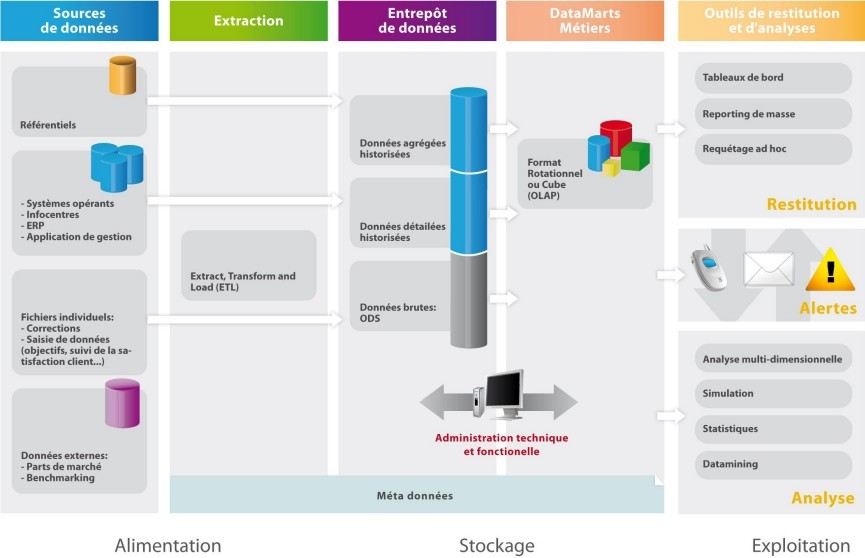
\includegraphics[width=1\linewidth]{./images/1}
\end{center}

\caption{Architecture d'un SID \citep{el2008ingenierie}}
\label{fig:1}

\end{figure}


\subsection{Sources de données}
\textcolor{black}{Les sources de données alimentent l’entrepôt de données. Elles sont regroupées en quatre catégories \citep{ponniah2001data} :}

\begin{itemize}
	\item  \begin{bf}Les données de production : \end{bf}ce sont les données provenant des différents systèmes opérationnels. Elles sont contenues dans des bases de  données transactionnelles et elles sont caractérisées par leur disparité (plusieurs technologies, environnements différents, …).
	\item  \begin{bf}Les données internes :  \end{bf}il s’agit des données concernant l’entreprise mais détenues par des employés ou des départements dans leurs  fichiers et base de données personnels, leur acquisition est de ce fait complexe. 
	\item  \begin{bf}Les données archivées : \end{bf}les données anciennes que le système opérationnel stocke périodiquement dans des fichiers ou base de données.  
	\item  \begin{bf}Les données externes : \end{bf} données externes à l’entreprise, il peut s’agir de statistiques d’agence externes, d’indicateurs de performance… nécessaires pour se situer par rapport à la concurrence et repérer les tendances du marché.
\end{itemize}
\subsection{Le processus ETL (Extraction, Transformation et Chargement)}
\textcolor{black}{Afin d’exploiter les données pour la prise de décision, il faut les rassembler dans une même zone. Et comme les données de l’entreprise, qu’elles soient homogènes ou hétérogènes, se trouvent dans plusieurs endroits alors on utilise un outil ETL pour les rassembler.}

\textcolor{black}{Selon \citep{polet12infor}, un ETL extrait, nettoie, et importe les données à partir de  différentes sources et les charge dans un entrepôt de données.}

\subsection{Les entrepôts et magasins de données}
\textcolor{black}{Grâce au processus ETL, les données sont stockées et organisées dans un entrepôt de données. Le concept d’entrepôt de données a été introduit car les bases de données transactionnelles ne  répondent pas aux besoins d’analyse.}
\subsubsection{Entrepôts de données}
\textcolor{black}{Kimball définit l’entrepôt de données comme étant « une copie des données transactionnelles d’une entreprise structurée de manière spécifique pour l’interrogation et l’analyse » \citep{kimball1996data}.}

\textcolor{black}{De son coté, Bill Inmon fournit la définition suivante :}

\textcolor{black}{« Un entrepôt de données est  une collection de données orientées sujet, intégrées, variant selon le temps et non volatiles, qui sert de support au processus de prise de décision des acteurs du management (les décideurs) » \citep{inmon1996building}.}

\textcolor{black}{Cette définition met l’accent sur les caractéristiques suivantes :}

\begin{itemize}
	\item  \begin{bf}Orientées Sujet : \end{bf}les données sont liées au métier de l’entreprise et organisées par fonction.
	\item  \begin{bf}Intégrée :  \end{bf}signifie que les données obtenues à partir de plusieurs systèmes opérationnels et externes doivent être réunies, ce qui implique la résolution de problèmes en raison de  différences de définition de données et de contenu, tels que les différences de format de données et la codification des données.
	\item  \begin{bf}Variant selon le temps : \end{bf}toutes les données d’un entrepôt sont identifiées par des périodes temporelles spécifiques, cela signifie qu’on garde l’historique de toutes les transactions.
	\item  \begin{bf}Non Volatiles :\end{bf}les données dans un entrepôt sont utilisées pour les interrogations et ne peuvent pas être modifiées. Donc, les opérations de mise à jour et suppression ne sont pas autorisées, et la lecture est la seule opération permise.
\end{itemize}

\textcolor{black}{Donc, un entrepôt de données est un référentiel centralisé qui stocke les données opérationnelles d’une manière spécifique et les rend disponibles et exploitables pour des fins d’analyse. }

\textcolor{black}{Les entrepôts sont souvent très volumineux et très complexes à concevoir, ils ont été divisés en petits entrepôts, faciles à créer et à entretenir, appelés  data marts  ou magasins de données.}

\subsubsection{Magasins de données (DataMart)}
\textcolor{black}{Un magasin de données est un extrait de l’entrepôt conforme à des besoins d’analyse particuliers et organisé selon un modèle adapté aux outils d’analyse et d’interrogation décisionnelle. Le magasin est généralement stocké au sein d’une base de données multidimensionnelle (BDM) \citep{tournier2007analyse}. Cela signifie qu’un magasin concentre sur les données d’un département dans l’entreprise.    }

\textcolor{black}{Pour une bonne gestion de données, l'entrepôt de données doit nécessairement disposer de métadonnées (données sur les données).}

\textcolor{black}{Les métadonnées d’un entrepôt de données se présentent sous trois catégories \citep{ponniah2001data} : 
	}


\begin{itemize}
	\item  \begin{bf}Métadonnées opérationnelles : \end{bf}Elles contiennent toutes les informations sur  les sources de données opérationnelles.
	\item  \begin{bf}Métadonnées d’extraction et de transformation :\end{bf}Elles contiennent  les fréquences d’extraction, les méthodes d’extraction, les  règles d’extraction, les  informations sur toutes les transformations opérées sur les données. 
	\item  \begin{bf}Métadonnées de l’utilisateur final : \end{bf}Elles permettent à l’utilisateur final de retrouver l’information dans l’entrepôt de données.
\end{itemize}
\subsubsection{Types de données stockées dans un entrepôt de données}
\textcolor{black}{Un entrepôt de données est articulé en quatre catégories de données, organisées selon un axe historique et un axe synthétique.  }

\textcolor{black}{L’axe synthétique établit une hiérarchie d’agrégation comprenant \citep{inmon2002building} :}


\begin{itemize}
	\item  \begin{bf}Les données détaillées : \end{bf} elles proviennent des systèmes opérationnels et représentent les évènements les plus récents. Seules les données qui servent au processus décisionnel sont stockées dans l’entrepôt.
	\item  \begin{bf}Les données agrégées : \end{bf}Elles synthétisent les données détaillées et correspondent à des éléments d’analyse représentatifs des besoins utilisateurs. Elles ont pour but de faciliter la navigation suivant les besoins décisionnels et la restitution d’un résultat d’analyse ou de synthèse.
	\item  \begin{bf}Les données fortement agrégées : \end{bf}Elles synthétisent les données agrégées à un niveau supérieur.
	\end{itemize}


\textcolor{black}{L’axe historique comprend \begin{bf} les données détaillées historisées \end{bf}représentant les évènements passés.}

\subsubsection{Modélisation des entrepôts de données}
\textcolor{black}{La modélisation d’un entrepôt de données est le processus permettant de mettre en place un entrepôt de données. Il existe plusieurs approches pour mettre en place un entrepôt de données. Cependant, trois approches sont les plus répandues. Il s’agit de l’approche d’Inmon, l’approche de Kimball et l’approche Data Vault.}

\textcolor{black}{L’étude et la comparaison de ces trois approches sont abordées dans les deux prochains chapitres.}

\subsection{Outils d’analyse et de restitution de données}
\textcolor{black}{Le dernier niveau correspond à la partie visuelle et accessible par les utilisateurs du système décisionnel. Il est l’élément le plus important pour l’utilisateur, car il lui permet d’exploiter, d’analyser et de restituer les données stockées. On distingue à ce niveau plusieurs types d’outils différents parmi eux :}
\subsubsection{Tableau de bord}
\textcolor{black}{Plusieurs auteurs ont donné une définition au tableau de bord. Nous citons celle donnée par \citep{berland2004mesurer}:}

\textcolor{black}{Le tableau de bord est « un outil d’aide à la décision et  un ensemble d’indicateurs peu nombreux (cinq à dix) conçus pour permettre aux gestionnaires de prendre connaissance de  l’état et de l’évolution des  systèmes qu’ils pilotent et d’identifier les tendances qui les  influencent sur un horizon cohérent avec leurs fonctions ».}

\textcolor{black}{Les décideurs au sein d’une entreprise ont un ou plusieurs objectifs à atteindre. Le décideur à l’aide du tableau de bord adapte ses ordres et mesures de fonctionnement effectués pour réduire au maximum les écarts constatés entre les mesures et les objectifs à atteindre.}

\subsubsection{Reporting}
\textcolor{black}{Le reporting est l’ensemble des comptes rendus permettant à une entreprise de suivre  son activité. Cela permet à l’entreprise de s’évaluer grâce à la création périodique de  rapports et de bilans analytiques sur son activité. Ces rapports sont souvent destinés au  manager ou au corps exécutif \citep{polet12infor}.}
\textcolor{black}{Le but de ces rapports et bilans réguliers est de faire un point ponctuel sur la  stratégie de l’entreprise et ainsi permettre d’évaluer les moyens mis en œuvre. Mais ils fournissent également une aide à la décision pour les choix stratégiques et économiques de l’entreprise \citep{polet12infor}.}
\subsubsection{Analyse OLAP }
\textcolor{black}{Une caractéristique fondamentale du modèle multidimensionnel de l’entrepôt de données est qu'il permet de visualiser les données à partir de plusieurs points de vue et à plusieurs niveaux de détail.}

\textcolor{black}{Les opérations OLAP permettent de matérialiser ces perspectives ainsi que les niveaux de détails en exploitant les dimensions et leurs hiérarchies, fournissant ainsi un environnement d'analyse interactive des données.}

\textcolor{black}{D’après \citep{tournier2007analyse}, « les magasins de données reposent sur une modélisation multidimensionnelle des données extraites de l’entrepôt. Ceci permet de les représenter sous la forme de points dans un espace à plusieurs dimensions avec la métaphore de cube ou d’hypercube de données. Cette modélisation permet l’expression d’analyses en ligne (OLAP) multidimensionnelles. »}
\subsubsection{Data Mining}
\textcolor{black}{DM est l'exploration de données historiques (généralement de grande taille) à la recherche d'un modèle cohérent et /ou d'une relation systématique entre les variables. Elle est ensuite utilisée pour valider les résultats en appliquant les modèles détectés à de nouveaux sous-ensembles de données \citep{berry2000mastering}.}

\textcolor{black}{Selon \citep{fayyad1996advances}, l'exploration de données peut être divisée en deux tâches: tâches prédictives et tâches descriptives. Le but ultime de l'exploration de données est la prédiction; par conséquent, l'extraction de données prédictives est le type le plus commun de l'exploration de données et est celui qui a le plus d'application à des entreprises car les rendements d'extraction de données  peuvent ouvrir les yeux d'une entreprise à de nouveaux marchés, de nouvelles façons d'atteindre les clients et de nouvelles façons de faire des affaires. }

\section*{Conclusion}
\addcontentsline{toc}{section}{Conclusion}
\textcolor{black}{Les systèmes décisionnels occupent une place importante dans les entreprises vu qu’ils soutiennent les dirigeants pour prendre des décisions au bon moment.} 

\textcolor{black}{L’entrepôt de données est le cœur de l’architecture décisionnelle.  Il est alimenté à partir de données sources grâce aux outils d’ETL. Ces données deviennent alors exploitables à l’aide d’outils d’analyse et de restitution.}

\textcolor{black}{Le chapitre suivant est consacré à l’étude des approches de modélisation des entrepôts de données.}

% % % % % % % % % % % % % % % % % % % % % % % % % % % % % % % % % % % % % % % % % % % % % % % % % % % % % % % % % % % % % %
% % % % % % % % % % % % % % % % % % % % % % % % % % % % % % % % % % % % % % % % % % % % % % % % % % % % % % % % % % % % % %
% % % % % % % % % % % % % % % % % % % % % % % % % % % % % % % % % % % % % % % % % % % % % % % % % % % % % % % % % % % % % %

























\chapter{Approches de modélisation des entrepôts de données}
\section*{Introduction}
\addcontentsline{toc}{section}{Introduction}
\textcolor{black}{Afin de construire un entrepôt de données pour une entreprise, le choix des méthodes et outils de conception et de maintenance est une étape primordiale et très importante.}

\textcolor{black}{Depuis des décennies, deux approches classiques étaient en rivalité rude quant à la modélisation des entrepôts de données. L’approche de modélisation par sujet et normalisation préconisée par son inventeur Inmon et l’approche de modélisation dimensionnelle de Kimball.}

\textcolor{black}{Ces dernières années, une nouvelle approche est entrée fortement en compétition et attire l’attention des entreprises jour après jour. Elle s’agit de l’approche Data Vault développée par son inventeur Dan Linstedt.
Dans ce chapitre, nous allons étudier chaque approche : sa philosophie, son architecture et la méthodologie pour la mettre en place.}


\section{Approche d’Inmon}



\textcolor{black}{Cette approche est créée par Bill Inmon\footnote{http://www.inmoncif.com/about/} dans les années 90 pour répondre au besoin des entreprises et leur permettre de développer leurs systèmes décisionnels. Elle permet le stockage de l’intégralité des évènements de l’entreprise et engage des ressources et moyens importants pour la réaliser.}

\textcolor{black}{L'approche d'Inmon est basée sur les schémas Entité-Association des systèmes opérationnels. Les données de l’entreprise sont chargées sans connaitre à priori les besoins des utilisateurs \citep{denis2008}, C’est pourquoi cette approche est qualifiée de « piloter par les données ».}



\subsection{Philosophie de l’approche}
\textcolor{black}{Inmon, informaticien américain et inventeur de l’approche, définit l’entrepôt de données comme étant une collection de données orientées sujet, intégrées, variant selon le temps et non volatiles (Voir chapitre 01).}
\textcolor{black}{Pour la construction d’un entrepôt de données, Inmon propose une méthodologie guidée par les données. Cette méthodologie est présentée en trois parties qui sont :}

\begin{enumerate}
	\item \textbf{Meth 1 :} pour le développement des systèmes opérationnels.
	\item \textbf{Meth 2 :} pour le développement des entrepôts de données.
	\item \textbf{Meth 3:} pour la description de l’usage de l’entrepôt de données.
\end{enumerate}

\textcolor{black}{L’architecture de l’entrepôt proposée par Inmon [Figure \ref{fig:2}] inclut tous les systèmes d’informations de l’entreprise avec leurs bases de données au lieu de ne considérer que des fragments d’information. Inmon divise l’environnement des bases de données de l’entreprise en quatre niveaux à savoir : opérationnel, atomique (Entrepôt de données), départemental (magasins de données) et individuel.}

\textcolor{black}{Les trois derniers niveaux constituent l’entrepôt alors que le premier niveau (opérationnel) supporte les opérations quotidiennes et contient les données transactionnelles de l’entreprise. Ces données sont ensuite transformées et chargées dans l’entrepôt de données atomique en utilisant un processus ETC (Extraction, transformation et chargement). Selon le besoin des différents départements de l’entreprise, les données détenues par le niveau départemental sont orientées sujet et toujours cohérentes car elles proviennent du même entrepôt.}

\textcolor{black}{Inmon considère que l’entrepôt et le magasin sont physiquement dissociés. L’entrepôt possède sa propre existence physique et il est orienté stockage, traçabilité et évolutivité par rapport à de nouveaux besoins. Les magasins possèdent aussi leur propre existence physique et proposent des structures orientées performances de restitution en réponse aux besoins exprimés par l’utilisateur.}

\textcolor{black}{Le dernier niveau est créé par les utilisateurs quand ils analysent et exploitent les données chargées dans les magasins de données (Analyse OLAP, Reporting, Tableaux de bord, etc.).}



\begin{figure}[H]
\begin{center}
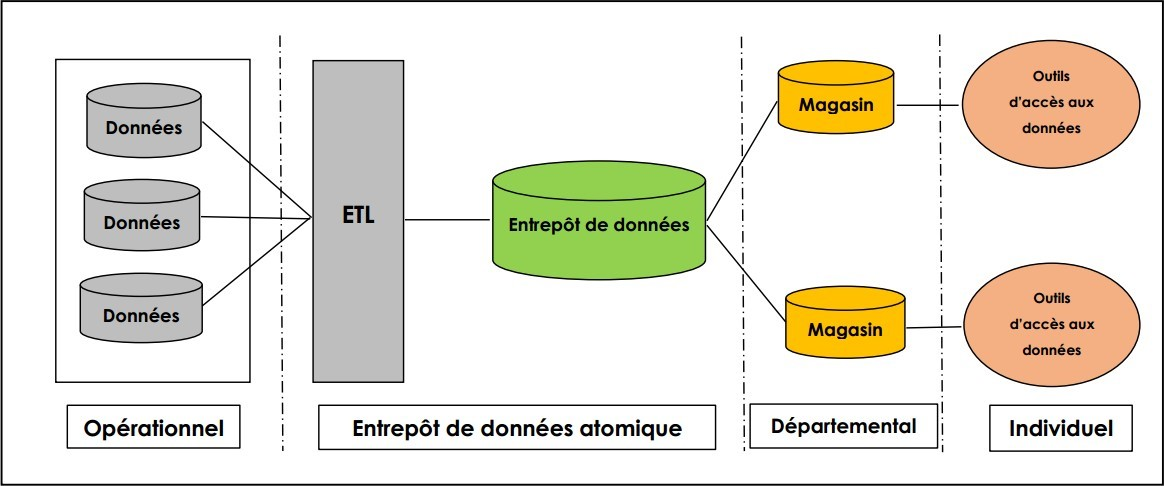
\includegraphics[width=1\linewidth]{./images/2}
\end{center}
\caption{Architecture de l’entrepôt de données. Adaptée de \citep{weir2008}}
\label{fig:2}
\end{figure}




\textcolor{black}{
L’approche d’Inmon est très complexe et requiert une connaissance approfondie de l’entreprise. Elle maximise la participation des professionnels des technologies de l’information. Cependant, les utilisateurs finaux sont faiblement impliqués dans le processus d’élaboration de l’entrepôt de données.}

\textcolor{black}{Dans notre étude, nous nous intéressons à la deuxième partie de la méthodologie (Meth 2) qui présente les étapes de développement d’un entrepôt de données.}


\subsection{Développement de l’entrepôt de données}

\textcolor{black}{Pour mettre en œuvre un entrepôt de données, Inmon propose une méthodologie de développement spirale (Meth 2) qui requiert les procédures suivantes :}


\begin{figure}[H]

\begin{center}
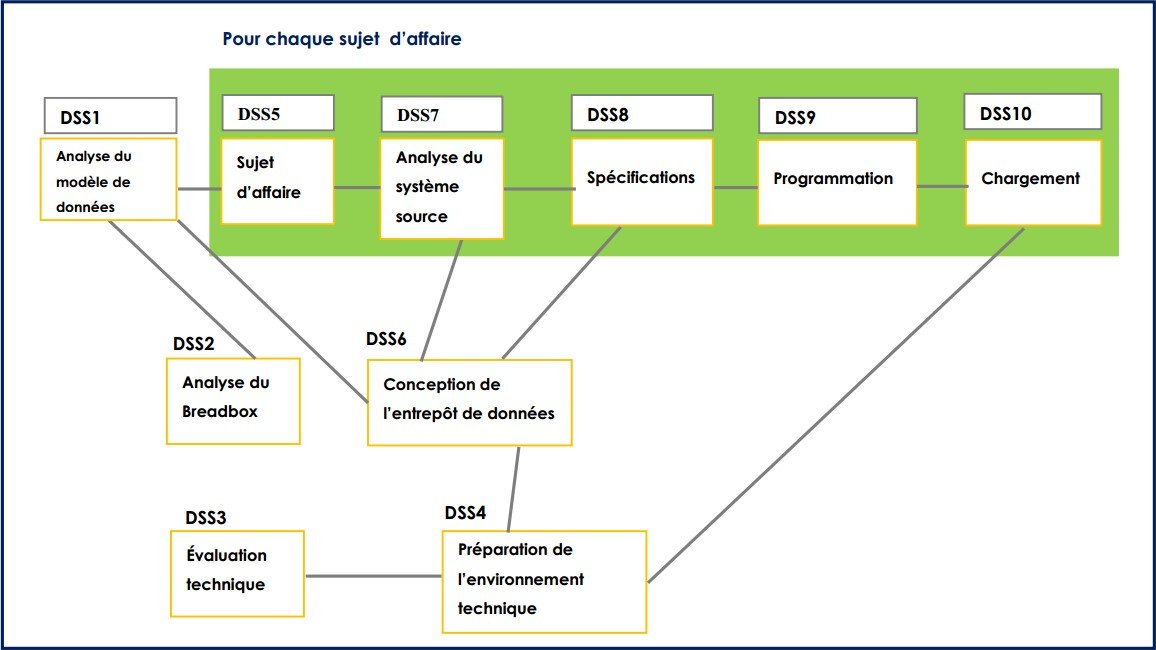
\includegraphics[width=1\linewidth]{./images/3}
\end{center}
\caption{Meth 2 d'Inmon. Reproduite \citep{inmon2002building}}
\label{fig:3}
\end{figure}



\subsubsection{Analyse du modèle de données}

\textcolor{black}{Le modèle de données de l’entreprise est le point de départ pour la mise en œuvre de l’entrepôt de données. A cet effet, il est important qu’il soit complet.}

\textcolor{black}{Pour établir ce modèle, Inmon propose trois niveaux de modélisation de données à savoir : }


\paragraph{Diagrammes d’Entité-Association(ERD) :}

\textcolor{black}{Pour la modélisation à haut niveau d’abstraction de données. Ce modèle, comme dans le développement des bases de données opérationnelles, consiste à identifier dans un premier temps les sujets d’affaires de l’entreprise(les entités) et dans un deuxième temps, identifier les relations qui existent entre ces entités.}

\textcolor{black}{Pour chaque département de l’entreprise qui veut utiliser l’entrepôt de données, on crée des ERD et l’ensemble constituera l’ERD de l’entreprise \citep{inmon2002building}.}

\textcolor{black}{La figure suivante montre un exemple d’un modèle de données de haut niveau.}


\begin{figure}[H]
\begin{center}
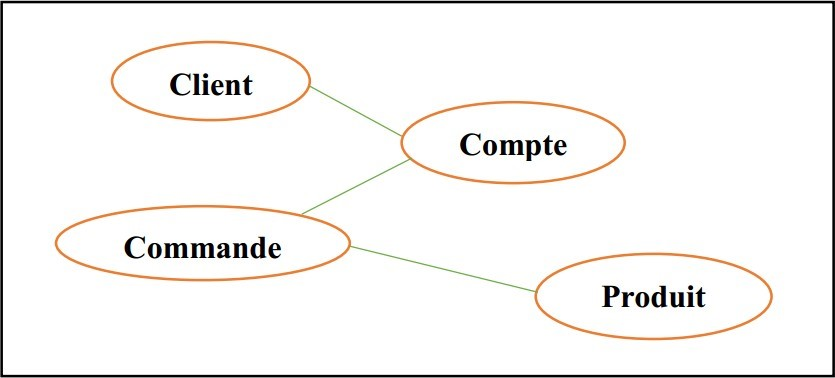
\includegraphics[width=0.5\linewidth]{./images/4}
\end{center}

\caption{Exemple d'un modèle ERD}
\label{fig:4}

\end{figure}

\paragraph{Data Item Set : }

\textcolor{black}{Le deuxième niveau de modélisation représente l’endroit où on trouve le maximum d’informations sur le modèle de données de l’entreprise. Pour chaque sujet d’affaire identifié dans l’ERD de l’entreprise, un DIS (acronyme de Data Item Set) sera créé. Ce niveau de modélisation contient des clés, des attributs, des sous-types, des groupements d’attributs, et des connecteurs.}

\textcolor{black}{Un DIS est constitué de quatre parties :}

\begin{enumerate}
	\item \textbf{Premier groupement de données: }
	le premier groupement de données existe seulement pour chaque sujet d’affaire (entité). Il contient les attributs (clé primaire et autres attributs) qui existent une seule fois pour chaque entité, Autrement dit, les caractéristiques qui identifient seulement l’entité qu’on est en train de modéliser. Si l’entité ou notre sujet d’affaire est ‘Personne’ alors le premier groupement va contenir le numéro de sécurité social de la personne(NSS) et autres attributs en relation directe avec l’entité.
	
	\item \textbf{Deuxième groupement de données: }	
	contient les données qui peuvent exister plusieurs fois pour chaque entité ou sujet d’affaire. Supposons que l’entité modélisée est ‘Personne’ alors il va y avoir multiples ensembles de données concernant son éducation, ses fils, etc. Ces données peuvent être des clés, clés étrangères ou autres attributs, mais la clé à ce niveau peut ne pas être unique.
	
	\item \textbf{Connecteur: }	
	le connecteur met en évidence les relations entre les sujets d’affaires.
	\item \textbf{Types de données: }	
	cette partie montre les différents types de l’entité, c’est-à-dire, pour une entité donnée on détermine les types qui peuvent exister selon des critères de classification. Par exemple, Si l’entité est ‘Client’ et le critère est la fidélité alors les différents types de données peuvent être client fidèle et client potentiel.
	
	\end{enumerate}
	
	
	
\textcolor{black}{La figure suivante montre un exemple d’un modèle DIS.}

\begin{figure}[H]

\begin{center}
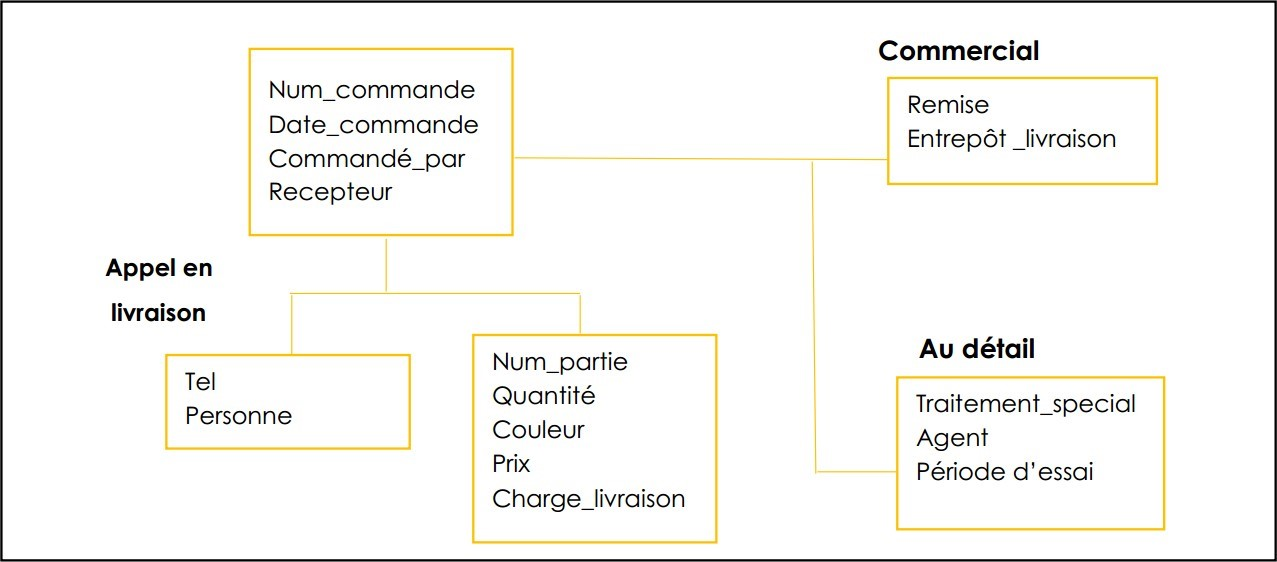
\includegraphics[width=0.7\linewidth]{./images/5}
\end{center}

\caption{Exemple d'un modèle DIS. \citep{inmon2000}}
\label{fig:5}

\end{figure}



\textcolor{black}{Nous constatons dans l’exemple le DIS relatif à l’entité Commande. Une commande a un ensemble d’informations basiques comme le numéro de la commande et la date. Il y a différents types de commande comme les commandes commerciales et les commandes au détail. Chaque commande peut avoir multiples occurrences des éléments qui ont été commandés, et peut avoir ou non des informations spécifiques comme la personne à appeler à la livraison.}

\paragraph{Le modèle physique}
	
\textcolor{black}{C’est le dernier niveau de modélisation. Il est créé en se basant sur le modèle de données du second niveau. Pour chaque partie du DIS, il y aura un modèle de données physique unique et séparé. Ce modèle ressemble aux tables relationnelles.}

\subsubsection{Analyse du breadbox}

\textcolor{black}{L’analyse du breadbox s’inscrit dans le processus des grandes estimations du système décisionnel. Parfois, le volume de l’entrepôt de données pose problème, c’est pourquoi il est préférable de le connaitre dès le début. Cette analyse permet de mettre en lumière ce problème et essaie d’estimer le volume de l’entrepôt de données. Elle considère principalement les niveaux de granularité de données (niveau de détail) car c’est la raison majeure qui influe sur la taille de l’entrepôt.}

\subsubsection{Evaluation technique }

\textcolor{black}{« Les exigences techniques pour le management et le traitement de données dans l’environnement opérationnel sont totalement différentes de celles pour manager l’entrepôt de données.» \citep{inmon2002building}.}

\textcolor{black}{
Cette phase consiste à établir une configuration architecturale de l’entrepôt de données. Le format d’évaluation dépend des décisions de l’entreprise et de ce qu’elle détient en termes d’équipements. Aucun format d’évaluation n’est donc prédéfini. Néanmoins pour un entrepôt couronné de succès, ses fonctionnalités doivent respecter les standards suivants :
}

\begin{itemize}

\item  Manipulation d’un énorme volume de données.
\item  Flexibilité d’accès aux données.
\item  Organisation des données de l’entrepôt en respectant le modèle de données de l’entreprise.
\item Capacité d’interaction avec une multitude de technologies.

\end{itemize}

\subsubsection{Préparation de l’environnement technique}

\textcolor{black}{« Une fois la configuration architecturale définie, on identifie techniquement comment l’architecture peut être accommodée. » \citep{inmon2002building}. \citep{inmon2002building} liste les problèmes devant être traités :}

\begin{itemize}
\item Comment le réseau des technologies d’information de l’entreprise va être affecté par le trafic accru à cause de l’entrepôt de données ?
\item Comment minimiser les conflits entre les applications existantes ?
\item Quel est le type de connectivité réseau nécessaire ?
\item Quel est le volume de traitement prévu ?

\end{itemize}

\subsubsection{Analyse des sujets d’affaires}

\textcolor{black}{Cette étape est considérée comme la première étape expérimentale dans le processus de développement de l’entrepôt de données.}

\textcolor{black}{
Le processus d’analyse des sujets d’affaires est fortement lié à la compréhension et à la maitrise du modèle de données de l’entreprise vu qu’on se base principalement sur ce dernier pour dégager les éléments de données qui vont être chargées dans l’entrepôt de données. Il est conseillé que le sujet d’affaire soit suffisamment large pour être significatif et suffisamment petit pour être applicable.}

\subsubsection{Conception de l’entrepôt de données}

\textcolor{black}{La conception est la phase la plus importante dans le processus de développement de l’entrepôt de données, c’est pourquoi le modèle de données et l’analyse des sujets d’affaires sont des étapes critiques pour un entrepôt réussi. }

\textcolor{black}{Pour construire l’entrepôt de données, un certain nombre de transformations seront faites sur le modèle de données de l’entreprise. Nous abordons dans ce qui suit les transformations qui seront appliquées :}

\begin{enumerate}
\item \textbf{Les données purement opérationnelles sont supprimées entièrement du modèle de données de l’entrepôt:} Il s’agit de toutes les données qui n’ont pas d’intérêt pour les décideurs.


\begin{figure}[h!]

\begin{center}
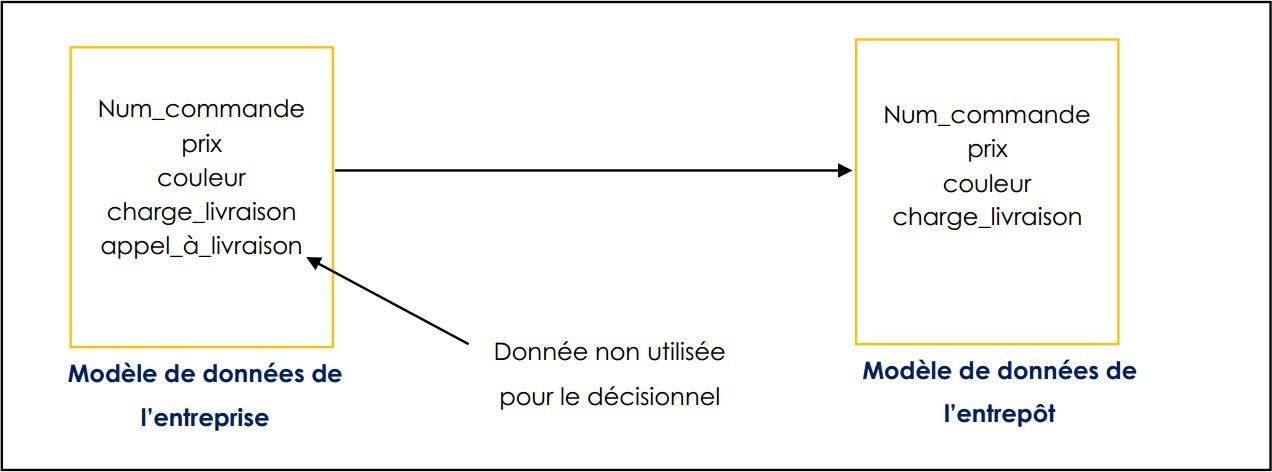
\includegraphics[width=0.7\linewidth]{./images/6}
\end{center}

\caption{Suppression de données non utilisées pour le décisionnel. \citep{inmon2000}}
\label{fig:6}

\end{figure}


\item \textbf{L’ajout d’un élément de temps} à la clé de l’entrepôt de données s’il n’existe pas.

\begin{figure}[H]
\begin{center}
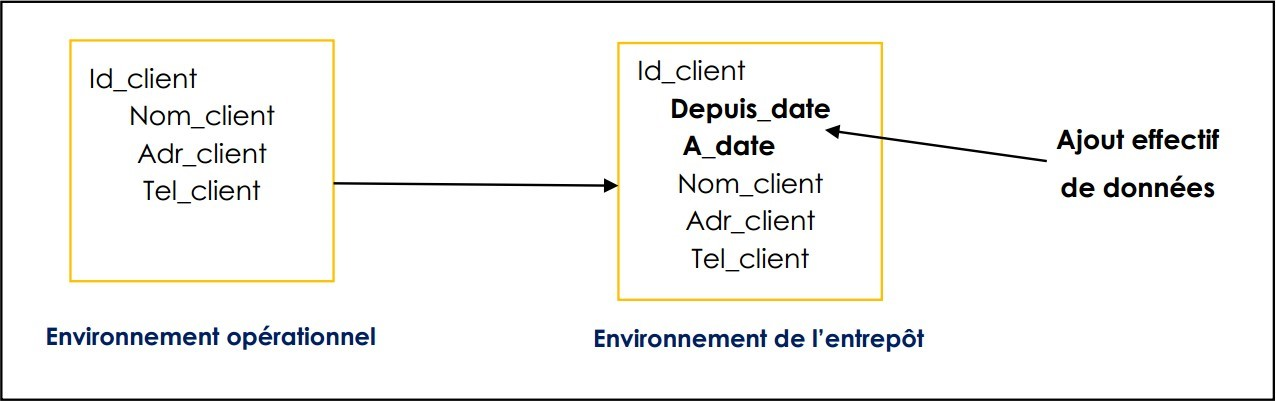
\includegraphics[width=0.7\linewidth]{./images/7}
\end{center}

\caption{Ajout de l'élément temps}
\label{fig:7}

\end{figure}



\item \textbf{L’ajout de données dérivées qui sont populaires et calculées.} La figure suivante montre un exemple d’ajout de données dérivées.

\begin{figure}[H]
\begin{center}
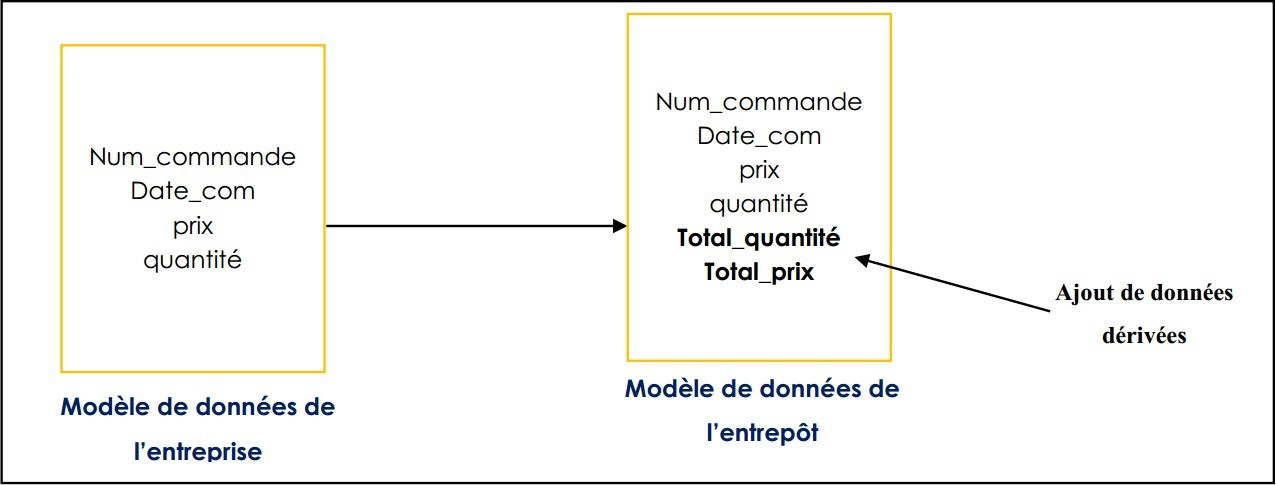
\includegraphics[width=0.7\linewidth]{./images/8}
\end{center}

\caption{Ajout de données dérivées}
\label{fig:8}

\end{figure}


\textcolor{black}{L’ajout de données dérivées réduit le taux de calcul requis et améliore la crédibilité de données dans l’entrepôt.}


\item \textbf{Accommodation des différents niveaux de granularité de l’entrepôt de données : } Parmi les caractéristiques principales d’un entrepôt de données la granularité de données. Parfois le niveau de granularité ne change pas quand les données passent de l’environnement opérationnel à l’environnement de l’entrepôt de données. Dans d’autres cas, la granularité change et ce changement doit apparaitre dans le modèle de données de l’entrepôt de données.

\textcolor{black}{La figure suivante montre un exemple de changement du niveau de granularité.}


\begin{figure}[H]

\begin{center}
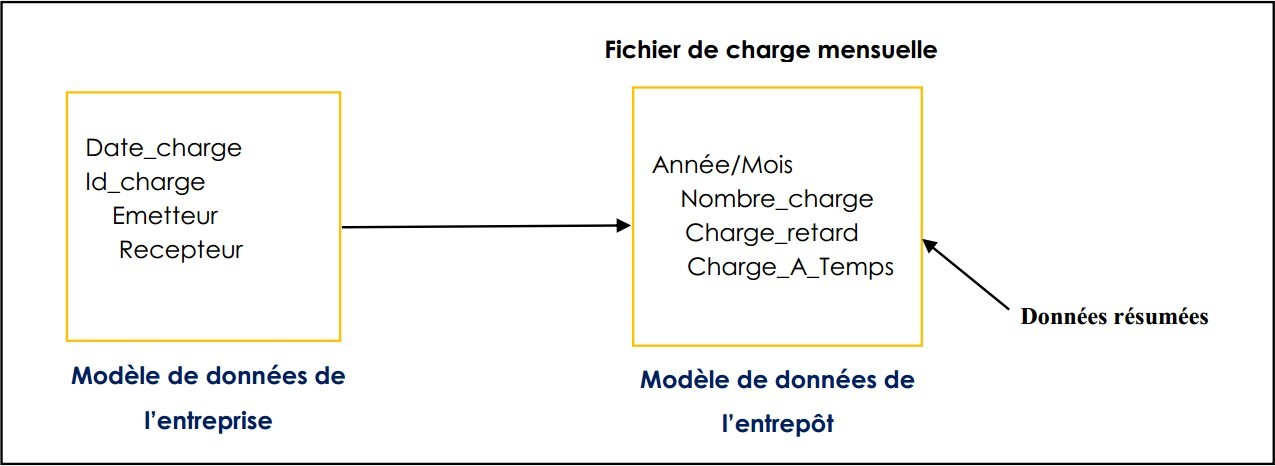
\includegraphics[width=0.7\linewidth]{./images/9}
\end{center}
\caption{Changement du niveau de granularité. \citep{inmon2000}}
\label{fig:9}

\end{figure}


\item \textbf{Fusion de données semblables de différentes tables en une seule table}: Cela permet de gagner en espace et en performance, mais la fusion ne se fait pas tout le temps et les conditions suivantes sont nécessaires \citep{inmon2000} :

\begin{itemize}

\item Les tables partagent une clé commune.
\item Les données des différentes tables sont fréquemment utilisées ensemble.
\item Le processus d’insertion de données est presque le même.

\textcolor{black}{Si aucune de ces conditions n’est présente alors aucune fusion de tables ne sera faite.} 

\end{itemize}

\item \textbf{Création des tableaux de données :} la redondance de données dans le modèle de données de l’entreprise n’est pas permise. Cela est dû au fait que les données sont normalisées. Par contre, l’entrepôt de données peut et devrait contenir des données répétées.

\item \textcolor{black}{ \textbf{Organisation de données selon leur degré de stabilité :}} C’est la dernière transformation à faire sur les données et qui vise à organiser les données dans l’entrepôt selon leur tendance au changement. L’organisation de données dans l’entrepôt est optimale quand les données d’une table changent tous du même rythme. Certaines tables contiennent des données qui changent lentement alors que d’autres contiennent des données qui changent rapidement.

\textcolor{black}{La figure suivante montre un exemple de cette transformation.}

\begin{figure}[H]

\begin{center}
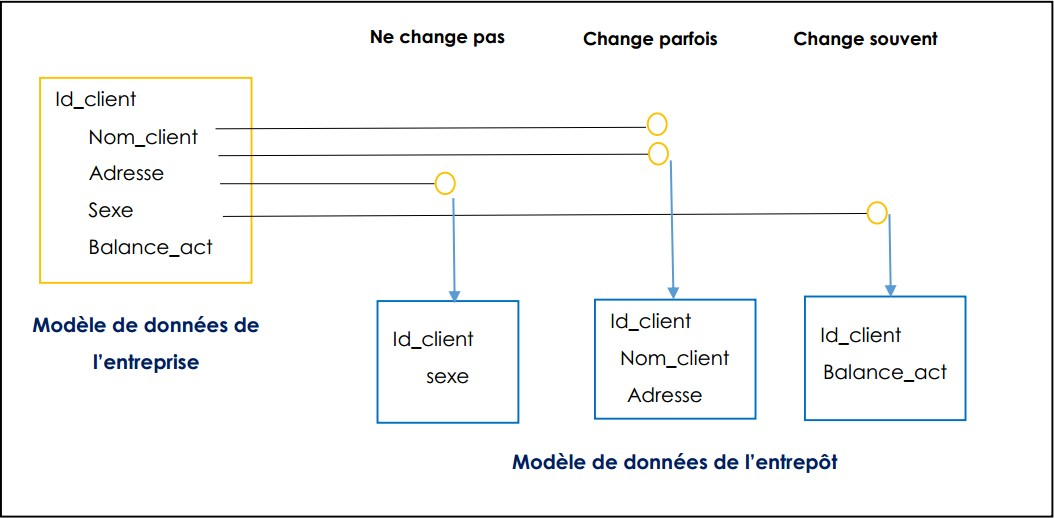
\includegraphics[width=0.7\linewidth]{./images/10}
\end{center}

\caption{Division de données selon leur degré de changement. \citep{inmon2000}}
\label{fig:10}

\end{figure}

\end{enumerate}
\subsubsection{Analyse des systèmes sources }
\textcolor{black}{Les sources de données de l’entreprise sont multiples et variées. Dans cette phase, l’équipe de projet est amenée à déterminer les sources de données qui vont alimenter l’entrepôt de données pour chaque sujet d’affaire identifié.}

\textcolor{black}{Pour déterminer les meilleures sources de données, Inmon propose les critères suivants :}

\begin{itemize}
\item 	Quelles sont les données les plus complètes ?
\item 	Quelles sont les données les plus exactes ?
\item	Quelles sont les données les mieux appropriées ?
\item	Quelles sont les données qui suivent la structure du modèle de données ?

\end{itemize}
\textcolor{black}{Inmon suggère dans l’analyse des sources de données de traiter les problèmes suivants:}

\begin{itemize}

\item	comment choisir à partir de plusieurs sources de données ?
\item	Comment procéder dans le cas où il n’y a pas de source ?
\item	Quelles sont les transformations à faire sur les données qui vont alimenter l’entrepôt de données ?

\end{itemize}

\textcolor{black}{Si on suit ces étapes proprement, alors le système source va être complet, approprié, exact et accessible. Il va aussi suivre la structure de l’entrepôt de données \citep{inmon2002building}.}

\subsubsection{Programmation}
\textcolor{black}{Cette phase inclut toutes les activités classiques de programmation comme :}

\begin{itemize}
\item	Pseudo-code.
\item	Codage.
\item	Compilation.
\item	Tests.
\end{itemize}
\textcolor{black}{A l’issue de cette étape, on obtient un code efficace, exact et complet.}

\subsubsection{Chargement}

\textcolor{black}{Cette étape correspond au chargement de données dans l’entrepôt de données. Dans un premier temps, on va charger juste la fraction de données dont on a besoin à ce stade.}

\textcolor{black}{Le chargement de données dans l’entrepôt ne se fait pas directement, il est précédé par un ensemble d’opérations telles que le nettoyage et le filtrage.}

\textcolor{black}{Le chargement d’un petit volume de données permet de faire les changements sur les données rapidement et facilement. Par contre, le chargement d’un volume important diminue considérablement la flexibilité de l’entrepôt.}

\textcolor{black}{Une fois les données chargées, les utilisateurs finaux peuvent utiliser les données stockées dans l’entrepôt et communiquer leurs réactions à l'équipe de développement, ce qui permettra le réajustement du système selon les exigences et les besoins de l'organisation. Ce n’est qu’après que le chargement d’un grand volume de données peut être envisagé.}

\section{Approche de Kimball}

\textcolor{black}{Kimball\footnote{http://www.kimballgroup.com/about-kimball-group/} a créé son approche dans les années 90 en proposant une nouvelle architecture, nouvelle vision et une modélisation novatrice de l’entrepôt de données.}

\textcolor{black}{Cette approche est basée sur le concept de la modélisation dimensionnelle. Kimball oppose la philosophie d’Inmon quant à l’isolation des utilisateurs finaux dans le processus d’élaboration de l’entrepôt. En effet, son approche implique fortement les utilisateurs finaux dès les premières phases du projet, C’est pourquoi cette méthode est appelée « piloter par les besoins utilisateurs ».}

\subsection{Philosophie de l’approche}

\textcolor{black}{Ralph Kimball propose une vision complètement différente pour les entrepôts de données. Il considère que l’entrepôt de données peut être vu comme un ensemble de magasins de données cohérents entre eux, s’appuyant sur des dimensions conformes partagées \citep{kimball2013data}. }

\textcolor{black}{L’intérêt de l’approche de Ralph Kimball est la rapidité de mise en place d’une solution décisionnelle adaptée aux besoins décrits. Ainsi, on gagne en temps de conception, réalisation, et investissements engagés. }

\textcolor{black}{Le modèle de Kimball diffère dans plusieurs points importants de l’approche traditionnelle de base de données relationnelle \citep{breslin2004data}. Une différence importante est que les entrepôts de données construites avec le modèle Kimball commencent par les tables au lieu des entités comme le modèle E/A. Cette question est examinée dans la section 2.2.3. }

\textcolor{black}{Une autre différence importante est que l'architecture globale dispose de plusieurs bases de données qui sont censés être hautement interopérables. Le bus de données est la principale caractéristique de conception qui rend cela possible  \citep{breslin2004data}.}

\textcolor{black}{
Plus de détails sur le bus de données et les dimensions conformes, veuillez voir respectivement les deux sections 2.2.3.3.3 et 2.2.3.3.4
}

\textcolor{black}{La figure suivante illustre l'architecture de l'entrepôt selon la vision de Kimball.} 

\begin{figure}[H]
\begin{center}
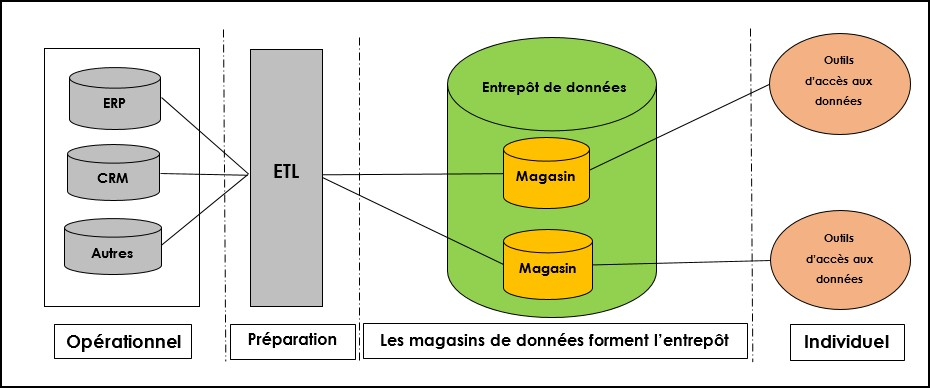
\includegraphics[width=1\linewidth]{./images/10bis}
\end{center}

\caption{L'architecture de l'entrepôt de données.}
\label{fig:23}

\end{figure}

\subsection{La modélisation dimensionnelle}

\textcolor{black}{La modélisation dimensionnelle de Kimball est une technique de conception logique qui vise à présenter les données dans un cadre normalisé intuitive et permet un accès de haute performance. Elle est fondamentalement basée sur les dimensions et les faits. Chaque modèle dimensionnel est composée d'une table avec une clé, appelé la table de faits, et un ensemble de petites tables appelées tables de dimension. }

\textcolor{black}{Pour comprendre toute la démarche de Kimball, nous allons la détailler à travers  le cycle de vie  Kimball (la figure ci-après), qui représente toutes les étapes garantissant une mise en place d’un entrepôt de données à partir de la planification, la définition de besoins et le passage par la modélisation jusqu’à la maintenance de l’entrepôt.  }

\subsection{Présentation du cycle de vie de Kimball}

\textcolor{black}{Selon Kimball, la finalité d’un entrepôt de donnée est de « fournir des informations pour soutenir la prise de décisions dans une entreprise» \citep{kimball2013data}. De ce fait, l’entrepôt de données est une base de données dédiée et utilisée dans le cadre de la prise de décision et de l'analyse décisionnelle. }

\textcolor{black}{Pour pouvoir concevoir un entrepôt de données selon l’approche de kimball, il est primordial de maitriser la modélisation dimensionnelle. }

\textcolor{black}{
Cette modélisation et d’autres notions nécessaires sont expliquées et détaillées dans le cycle de vie de kimball. 
La figure suivante représente le cycle de vie dimensionnel de Kimball illustrant les étapes nécessaires à la modélisation multidimensionnelle.}

\begin{figure}[H]
\begin{center}
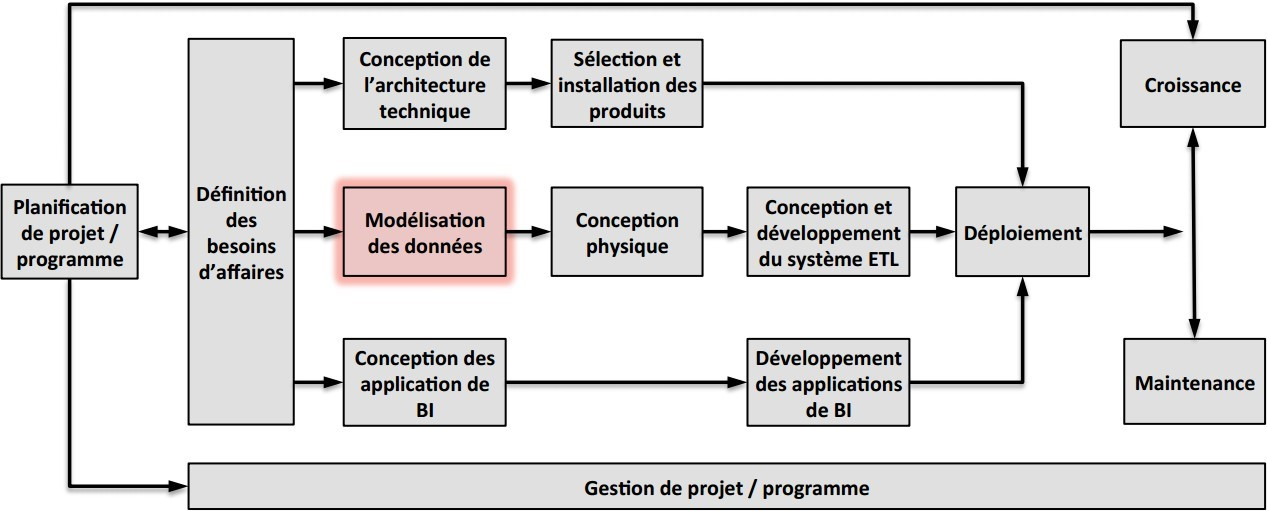
\includegraphics[width=0.9\linewidth]{./images/11}
\end{center}

\caption{L'architecture de l'entrepôt de données.\citep{kimball2013data}}
\label{fig:11}

\end{figure}


\textcolor{black}{Le cycle contient treize étapes. Nous constatons que la modélisation dimensionnelle est au cœur de ce cycle. Elle vient juste après la planification et la définition de besoins. Dans ce qui suit, nous détaillons les étapes du cycle de vie une par une.}

\subsubsection{	Planification du projet	}
\textcolor{black}{Le cycle de vie commence par la planification du projet. A ce stade on définit plusieurs points critiques qui anticipent l’échec ou le succès du projet \citep{kimball12data}):}

\begin{itemize}
\item	l’étendue du projet de l’entrepôt de donnée. 
\item	l’appréciation du niveau de maturité de l’organisation face à ce type d’approche.
\item	la justification fonctionnelle.
\item	les coûts associés.

\end{itemize}

\textcolor{black}{À partir de là, la planification du projet se concentre sur l’affectation des tâches, à leur durée et à leur séquencement. Le planning qui en découle identifie toutes les tâches associées au cycle de vie dimensionnel et mentionne les ressources impliquées. La planification du projet dépend des besoins, comme l’indique la flèche à double sens reliant ces deux activités.}

\subsubsection{Définition des besoins}

\textcolor{black}{Toutes les activités du cycle de vie est basée essentiellement sur la définition des besoins \citep{kimball2004data}. Cette méthodologie de collecte concernant les besoins de l'entreprise est différente des méthodologies traditionnels pilotée par les données \citep{inmon2005building}. Les analystes DW doivent comprendre les facteurs clés de l'entreprise afin de traduire avec succès les besoins de l'entreprise dans des considérations de conception \citep{kimball2008data}.}

\textcolor{black}{Voici les étapes suggérées par le cycle de vie Kimball concernant la collecte des besoins de l'entreprise \citep{kimball12data}:}

\begin{itemize}
\item	Préparer, conduire et résumer les interviews
\item	Examiner les résultats des interviews
\item	Etablir des priorités et l’enchaînement des étapes
\item	Exigences sur le niveau de finalité des projets
\item	Gestion des risques.  
\end{itemize}

\textcolor{black}{Une fois que tous les besoins de l'entreprise sont finalisés, les différents groupes de l'équipe peuvent commencer le travail sur des différentes parties; par exemple, un groupe peut commencer le travail sur la conception de l'architecture technique, et un autre groupe peut commencer le travail sur la modélisation dimensionnelle.}

\subsubsection{	Modélisation dimensionnelle des données}

\textcolor{black}{Popularisée par Ralph Kimball dans les années 90, cette modélisation est aujourd’hui reconnue comme la modélisation la plus appropriée aux besoins d’analyse et de prise de décision \citep{adamson2012mastering}.}

\textcolor{black}{La structuration et l’organisation des données offertes par la modélisation dimensionnelle facilitent la conceptualisation, la visualisation et l’analyse des données. Une vision multidimensionnelle des données met en avant le sujet analysé et les différentes perspectives d’analyse \citep{kimball2013data}. }

\textcolor{black}{Ce modèle multidimensionnel contient plusieurs concepts fondamentaux : la table de fait, les dimensions, les dimensions conformes ainsi que la matrice en bus. Nous les définissons dans cette section.}


\paragraph{La table de fait : }
\textcolor{black}{Une table de fait est une table qui contient les données observables (les faits) que l'on possède sur un sujet et que l'on veut étudier, selon divers axes d'analyse (les dimensions). Les « faits », dans un entrepôt de données, sont normalement numériques, puisque d'ordre quantitatif. Il peut s'agir du montant en argent des ventes, du nombre d'unités vendues d'un produit,...etc .}


\begin{figure}[H]
\begin{center}
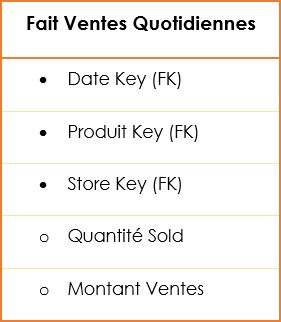
\includegraphics[width=0.3\linewidth]{./images/12}
\end{center}

\caption{La table de fait.\citep{dieng13etoile} }
\label{fig:12}

\end{figure}





\textcolor{black}{La figure précédente montre une table de fait possédant des clés étrangères (FK) qui se connectent à des clés primaires de dimension. Par exemple, la clé de produit dans la table de faits correspond toujours à une clé de produit spécifique dans la table de dimension du produit. Le “Montant Ventes” représente le fait à étudier.   }

\paragraph{La dimension :}

\textcolor{black}{Une dimension est une table qui contient les axes d'analyse (les dimensions) selon lesquels on veut étudier des données observables (les faits) qui, soumises à une analyse multidimensionnelle, donnent aux utilisateurs des renseignements nécessaires à la prise de décision \citep{ballard1998data}.}

\textcolor{black}{On appelle donc « dimension » un axe d'analyse. Il peut s'agir des clients ou des produits d'une entreprise, etc \citep{ballard1998data}.}


\begin{figure}[H]
\begin{center}
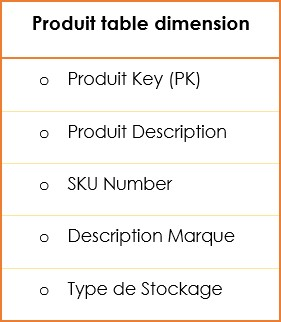
\includegraphics[width=0.3\linewidth]{./images/13}
\end{center}

\caption{La table de dimension Produit.\citep{dieng13etoile} }
\label{fig:13}

\end{figure}


\textcolor{black}{La figure montre les attributs décrivant les lignes de la table Produit.
D’autres attributs peuvent être ajoutés à la dimension. Ces attributs sont descriptifs et représentent l’information utile sur la dimension. Chaque table de dimension devrait contenir les colonnes suivantes:
}

\begin{itemize}
\item \textbf{Date effective :}	 c’est la date à laquelle l’enregistrement est créé.

\item \textbf{Date retrait :}	 C’est la date à laquelle l’enregistrement est retiré.

\item	\textbf{Indicateur effectif :} En général est ‘O’ si l’enregistrement est toujours actif (Date retrait non nulle), ‘N’ sinon.

\end{itemize}

\paragraph{Dimension conforme :}

\textcolor{black}{On parle de dimension conforme ou partagée (également appelée master dimensions ou common reference dimensions) lorsque la dimension est utilisée par les faits de plus d’un magasin de données. L’exemple le plus courant est la dimension « Produit » qui est utilisée par différents magasins de données «Finance », « Marketing »…\citep{breslin2004data}. L’avantage est :}

\begin{itemize}
\item	\textbf{la cohérence :} entre les différentes tables de faits.
\item	\textbf{l’intégration :} permet à l'entrepôt de données d'opérer comme un seul bloc uni.
\item	\textbf{La productivité :} favorise l'extension de l'entrepôt d'une itération de développement à l'autre.

\end{itemize}

\paragraph{	L’architecture en bus :	}

\textcolor{black}{L’architecture en bus de Kimball est un élément clé de l’approche multidimensionnelle de Kimball. Introduit dans les années 1990, la technologie et l'architecture de bus décompose le processus de planification de l’entrepôt de donnée en éléments gérables en se concentrant sur les processus métier de l'organisation, ainsi que les dimensions conformes.}

\textcolor{black}{L’architecture matrice en bus, illustré ci-dessous, est un outil de conception clé représentant les processus métier de base de l'organisation et les dimensions conformes associés.}

\begin{figure}[H]
\begin{center}
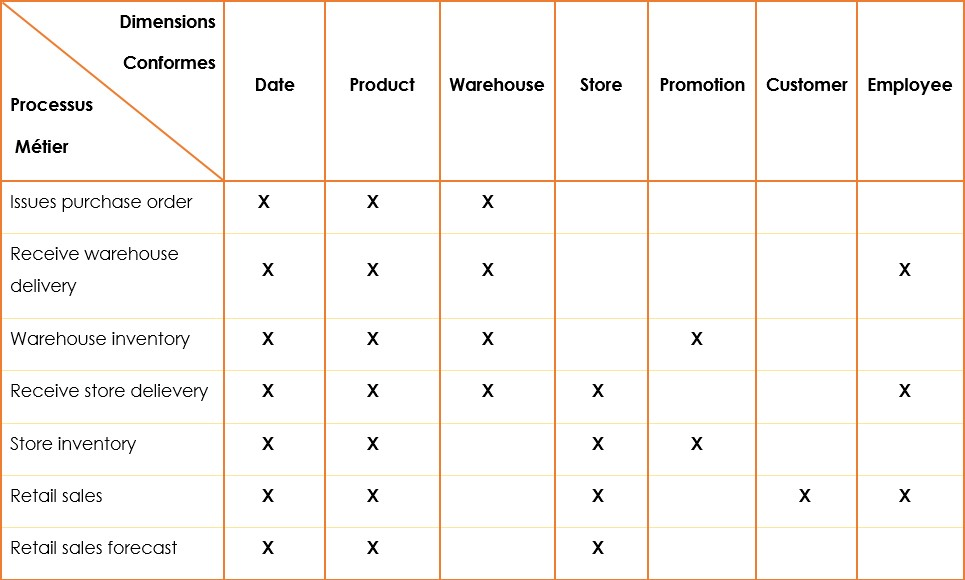
\includegraphics[width=0.9\linewidth]{./images/14}
\end{center}

\caption{Matrice de bus de Kimball \citep{kimb08bus}}
\label{fig:14}

\end{figure}

\textcolor{black}{D’une autre façon, la matrice de bus identifie les processus métiers clés d'une organisation, ainsi que leurs dimensions associées. L’influence de l’architecture en bus apparait clairement dans :}

\begin{itemize}

\item	\textbf{L’efficacité :} une seule copie d'une dimension  implique moins d'entretien.
\item	 \textbf{La cohérence :} une dimension conforme unique signifie la même chose partout où elle est utilisée.
\end{itemize}


\paragraph{Schémas pour modéliser :}

\textcolor{black}{Le schéma en étoile est conçu avec deux types de tables: tables dimensionnelles et tables de faits. Il existe de nombreuses variantes de schéma en étoile; par exemple, modèle avec plusieurs tables de faits et schémas de flocon de neige qui se posent lorsque une ou plusieurs dimensions ont une structure hiérarchique \citep{hoffer2009modern} .}
\textcolor{black}{Les trois schémas détaillés ici sont les schémas en Etoiles, flocons et constellations.  }

\subparagraph{Le schéma en étoile : }

\textcolor{black}{Chaque dimension est représentée par une table de dimension et les mesures par une table de faits qui référence les tables de dimension en utilisant une clé étrangère pour chacune d’elles.}

\begin{figure}[H]
\begin{center}
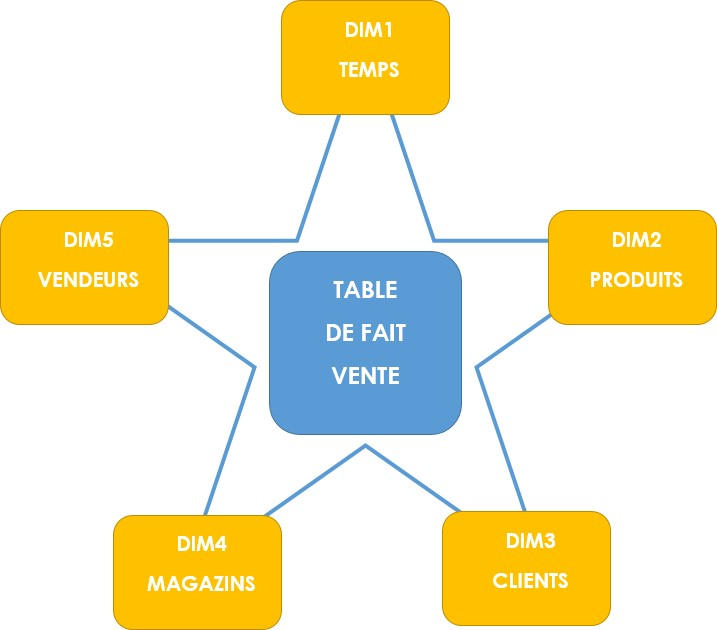
\includegraphics[width=0.5\linewidth]{./images/15}
\end{center}

\caption{Schéma en étoile.\citep{group16fg}
}
\label{fig:15}

\end{figure}


\subparagraph{Le schéma en flocon de neige :}

\textcolor{black}{C’est une extension du schéma en étoile. Le schéma en flocon est le résultat de la décomposition d’une ou plusieurs dimensions en plusieurs niveaux formant une hiérarchie. Les tables de dimensions sont ainsi éclatées en plusieurs tables.}

\begin{figure}[H]
\begin{center}
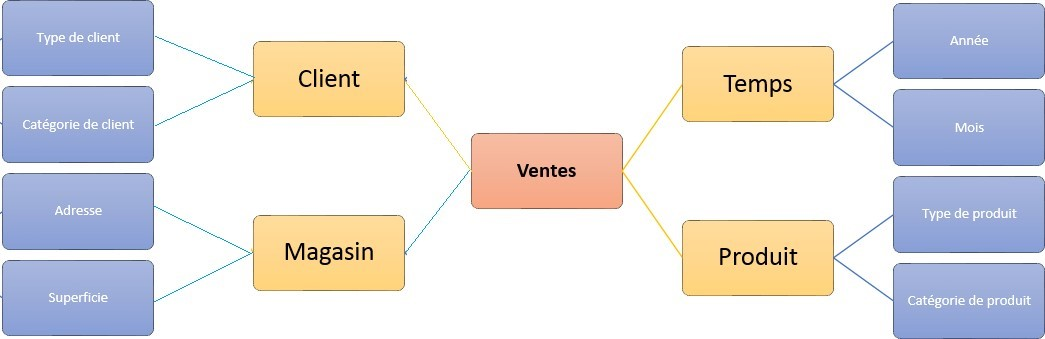
\includegraphics[width=0.7\linewidth]{./images/16}
\end{center}

\caption{Schéma en flocon de neige.\citep{group16fg}
}
\label{fig:16}

\end{figure}




\subparagraph{Le schéma en constellation :}

\textcolor{black}{C’est un schéma où plusieurs modèles dimensionnels se partagent les mêmes dimensions. Les tables de dimensions partagées par plusieurs tables de fait doivent être exactement les mêmes. }

\begin{figure}[H]
\begin{center}
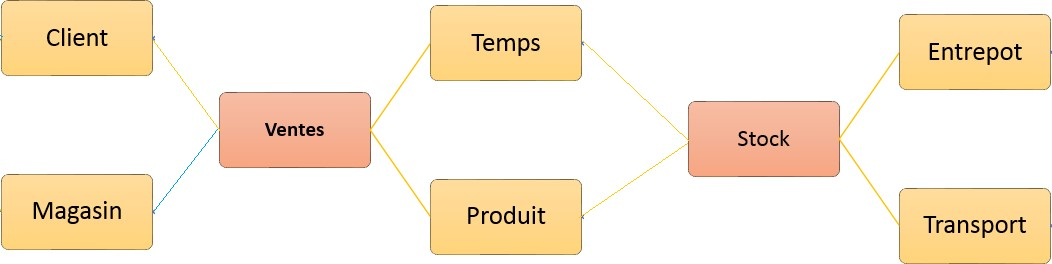
\includegraphics[width=0.7\linewidth]{./images/17}
\end{center}

\caption{Schéma en constellation. \citep{group16fg}
}
\label{fig:17}

\end{figure}


\subsubsection{Processus de modélisation dimensionnelle}

\textcolor{black}{Le processus de modélisation dimensionnelle est extrêmement itératif \citep{kimball12data}. Il est nécessaire à plusieurs reprises de tester la série des schémas contre la compréhension des besoins de l'entreprise \citep{kimball2004data}.}


\textcolor{black}{La modélisation dimensionnelle commence avec un modèle initiale. Cette phase  donne également une liste initiale des attributs avant sa validation. Les principaux objectifs de cette phase sont \citep{kimball12data}:}

\begin{itemize}
\item	créer un modèle qui répond aux besoins décisionnels de l'entreprise.
\item	vérifier que les données sont disponibles pour remplir le modèle.
\item	fournir à l'équipe d'ETL un point de départ solide et une orientation claire.

\end{itemize}

\textcolor{black}{Kimball et al. ont présenté quatre différents processus de conception dimensionnelle \citep{kimball2008data}:}


\begin{itemize}

\item \textbf{Choisir le processus d'affaires :} le concepteur de DW doit d'abord mettre en œuvre un seul magasin de données pour réduire la longue extraction et faciliter la tâche de conception, et ensuite appliquer la dimension conforme aux ensemble des magasins de données afin qu’on puisse plus tard les intégrer dans le bus de l'entrepôt de données.

\item \textbf{Déclarer le grain :} Lorsqu’on définit le grain des tables de faits, on doit être extrêmement précis.

\item \textbf{Identifier les dimensions :} Souvent le grain détermine un ensemble minimal de dimensions qui est nécessaire. 

\item \textbf{Identifier les faits :} La dernière étape est la sélection prudente des faits ou des mesures qui sont appropriées pour le processus de l'entreprise.

\end{itemize}


\subsubsection{Conception du modèle physique de données}

\textcolor{black}{On convertit dans cette phase les données recueillies lors de la phase de conception logique dans des bases de données physiques \citep{kimball2008data} .}

\textcolor{black}{La conception physique d’une base de données définit donc les structures physiques nécessaires pour l’implémentation des bases de données logiques. 
}

\textcolor{black}{ \citep{kimball2008data} recommande les étapes suivantes pour la conception physique:}

\begin{itemize}

\item \textbf{L'élaboration de normes :} les conventions de nommage, les normes de localisation de fichiers, les clés primaires et les clés étrangères…etc.

\item 	\textbf{Développer le modèle physique de données :} Définir la structure physique.

\item 	\textbf{Instancier base de données relationnelle :}  finalisé schéma en étoile ou schéma en flocon.


\end{itemize}

\subsubsection{Conception et développement de la zone de préparation des données}

\textcolor{black}{Kimball déclare dans son ouvrage que « la plupart des systèmes ont besoin d'un ensemble de tables de transit pour supporter les processus ETL » \citep{kimball12data}. L’extraction, la transformation et le chargement  prépare les données sources en vue de leur intégration puis de leur exploitation au sein de l’entrepôt de donnée.}

\textcolor{black}{ Un ensemble des processus qui nettoient, transforment, combinent, archivent, suppriment les doublons, est exécuté dans cette étape. De cette définition, la zone de préparation des données ne doit offrir ni service des requêtes, ni service de présentation. }

\textcolor{black}{Cette étape \citep{kimball2008data} consiste principalement en  la normalisation des données, le matching, la fusion des dossiers de la même entité qui sont tirées de sources différentes,  la production de données agrégées et le traitement des faits calculés…etc.}

\subsubsection{Définition de l’architecture technique}

\textcolor{black}{Les environnements des entrepôts de données nécessitent l’intégration de nombreuses technologies. Cette étape de définition donne une vision globale de la structure de l’architecture technique à mettre en œuvre. }

\textcolor{black}{Après avoir terminé la phase de conception de l'architecture, un modèle d'architecture technique de haut niveau est élaboré \citep{kimball2008data}.Le modèle de Kimball divise logiquement le système en deux parties (la Figure): les services de préparation (Back Room) et les services de requête (Front Room). }

 \begin{figure}[H]
 \begin{center}
 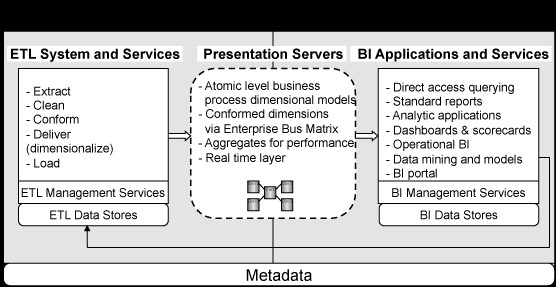
\includegraphics[width=0.9\linewidth]{./images/18}
 \end{center}
 
 \caption{L'architecture technique de Kimball.\citep{kimball16architec}
 }
 \label{fig:18}
 
 \end{figure}
 
 
\textcolor{black}{Le service de requête est la région où le processus d'acquisition de données est exécuté. La zone de transit de données est la zone où se passent les travaux d'extraction de données, de transformation, de chargement et de nettoyage.}

\textcolor{black}{L’architecture du  Back Room architecture est composée de \citep{kimball2008data}:}

\begin{itemize}

\item systèmes sources  opérationnels, systèmes ERP, ordinateurs de bureau des utilisateurs, fournitures extérieures, et fichiers plats

\item 	Un système ETL (Zone de préparation de données) : La zone chargée de contenir les données et d'effectuer le nettoyage et la transformation des données avant le chargement des données dans DW.

\end{itemize}

\textcolor{black}{La deuxième partie, qui est appelé les services de requête (Front Room), contient des applications de la BI. Le but principal de cette partie est de fournir l'accès à l'entrepôt de données par les utilisateurs pour exploiter le DW \citep{kimball2008data}.}

\textcolor{black}{L'architecture du Front Room fournit les services suivants \citep{kimball2008data}:}


\begin{itemize}

\item	\textbf{Requêtes, standards et rapports :} l'utilisateur peut accéder à l'information par des requêtes et des rapports.

\item	\textbf{Applications analytiques :} En plus de requêtes de base de données, il contient de puissants algorithmes d'analyse.

\item	\textbf{Les tableaux de bord :} Interfaces utilisées pour afficher les indicateurs clés de performance (KPI) textuelle et graphique.

\item \textbf{BI opérationnelle :}	 requêtes en temps réel de l'état de fonctionnement.

\item \textbf{Data mining et modèles :}	 l’exploitation de données historiques pour tirer des relations entre les variables.

\end{itemize}

\subsubsection{	Choix technologiques et mise en œuvre}

\textcolor{black}{À partir de l’étude de l’architecture technique, on évalue et sélectionne les composants, tels que la plate-forme matérielle, le système de gestion de base de données et les outils de préparation et d’accès aux données. }

\subsubsection{Développement de l’application utilisateur}

\textcolor{black}{Kimball recommande de définir une série d’applications standards destinée à l’utilisateur final.}

\subsubsection{Déploiement}

\textcolor{black}{Le déploiement est le point de convergence de la technologie, des données et des applications utilisateur accessibles à partir de postes de travail. }

\subsubsection{Maintenance et croissance}

\textcolor{black}{Une maintenance  d’un DW doit également assurer \citep{kimball2008data} :}

\begin{itemize}

\item	la gestion de l’entrepôt en continu et efficacement.
\item	la mesure périodique de son acceptation et ses performances.

\end{itemize}

\subsubsection{Gestion du projet}

\textcolor{black}{La gestion de projet garantit que les activités du cycle de vie dimensionnel restent sur la bonne voie et la bonne synchronisation entre elles. Comme le montre la figure du cycle de vie, les activités de gestion de projet sont étalées tout au long du cycle de vie. 
}

\textcolor{black}{La gestion de projet de Kimball concerne le contrôle de l’état d’avancement du projet, la détection et la résolution des problèmes et le contrôle des changements, afin de rester dans la limite des objectifs et du périmètre.}





\textcolor{black}{Après avoir identifié les nouveaux besoins des utilisateurs, on revient au début du cycle de vie, en prenant appui sur ce qui a déjà été mis en place dans l’environnement de l’entrepôt de données et en se penchant sur les nouveaux besoins. }


\section{Approche Data Vault}

\textcolor{black}{Au début des années 2000, Dan Linstedt\footnote{http://it.toolbox.com/people/dlinstedt/}  est entré dans la compétition en proposant une troisième approche dite « modélisation Data Vault » (par voûtes de données). Cette modélisation est qualifiée de mitoyenne située entre les deux approches de Kimball et Inmon. Elle est particulièrement adaptée à l'audit de données, à la traçabilité de la donnée et à la résistance au changement de la structure de données.}

\textcolor{black}{Cette approche palie plusieurs problèmes auxquels font face les deux approches classiques. Le problème majeur est le re-engineering en cas du changement du business}

\subsection{Définition du Data Vault}

\textcolor{black}{Dan Linstedt, informaticien américain et inventeur de l’approche, définit le Data Vault comme étant « un ensemble de tables normalisées orientées détail, suivant l’historique, liées de manière unique et qui supportent un ou plusieurs secteurs fonctionnels de l’entreprise \citep{3}. Autrement dit, c’est une approche mitoyenne qui prend le meilleur de la 3éme  forme normale (3NF) d’Inmon et le schéma en étoile de Kimball.}

\subsection{Philosophie de l’approche}

\textcolor{black}{Selon Linstedt, la modélisation 3NF d’Inmon et la modélisation dimensionnelle de Kimball connaissent une grande faiblesse quand le volume de données augmente. De ce fait, une nouvelle approche de modélisation s’impose.}



\textcolor{black}{La modélisation d’entrepôt dans les deux approches classiques se base uniquement sur une architecture de données. Data Vault considère la notion d’architecture de processus dans la modélisation. En effet, Les structures de données sont déterminées selon une modélisation relationnelle et selon une notion de processus selon la fonction de la donnée.\citep{4}}


\textcolor{black}{Data Vault s’intéresse aux changements dans les processus et structures de données plutôt que le changement dans les fonctions d’affaires \citep{4}.}


\textcolor{black}{Les caractéristiques principales du Data Vault sont les suivantes \citep{4} :}

\begin{itemize}

\item Les informations structurelles sont séparées des informations descriptives (attributs) pour des raisons de flexibilité et évitement du re-engineering en cas du changement.

\item 	Le Data Vault permet un chargement parallèle de données.

\item 	Les données ne sont pas transformées ni filtrées. L’approche permet de tracer la source des données.

\item 	Les données ne sont jamais modifiées, elles restent intactes.

\item	L’accès au Data Vault est restreint, sa structure ne permet pas une exploitation finale de données.

\end{itemize}

\textcolor{black}{Le Data Vault est une approche riche et solide. Elle est née pour promouvoir la flexibilité, l’évolutivité et la productivité de l’entrepôt de données.}

\subsection{Composants du modèle Data Vault}

\textcolor{black}{Dans le modèle Data Vault, on distingue trois types d’entités : les hubs, les liens et les satellites.}

\subsubsection{	Hub  }

\paragraph{	Définition du hub :}

\textcolor{black}{Les hubs sont définis par une liste unique des clés d’affaires (clés naturelles) qui identifient un concept utilisé par l’organisation tel que Client et Produit. Ces clés sont les piliers de tout le modèle et sont vitales pour les entreprises afin de suivre, localiser et identifier leur information. Les hubs constituent le point de raccordement entre les différents secteurs de l’organisation\citep{awel2014}.}

\textcolor{black}{Parfois ces clés d’affaires se trouvent dans les bases de données des systèmes transactionnels en tant que clés primaires.}

\textcolor{black}{Il est impératif que les clés d’affaires aient une unicité historique et générale, c’est-à-dire qu’il ne faut jamais utiliser la clé d’affaire dans différents secteurs de l’organisation pour signifier des choses différentes ou de les réutiliser\citep{qosqo12}.}

\textcolor{black}{On peut compléter chaque clé avec une ou plusieurs métadonnées comme son origine et sa date d'extraction.}

\paragraph{Structure du Hub :}

\textcolor{black}{L’entité hub est composée de ces éléments nécessaires : La clé d’affaire, la date du chargement, la source d’extraction et une clé de substitution (surrogate key en anglais) pour éviter les problèmes de performance liés aux clés complexes \citep{awel2014}.}

\textcolor{black}{La figure suivante montre la structure de l’entité hub et un exemple.}

\begin{figure}[H]
\begin{center}
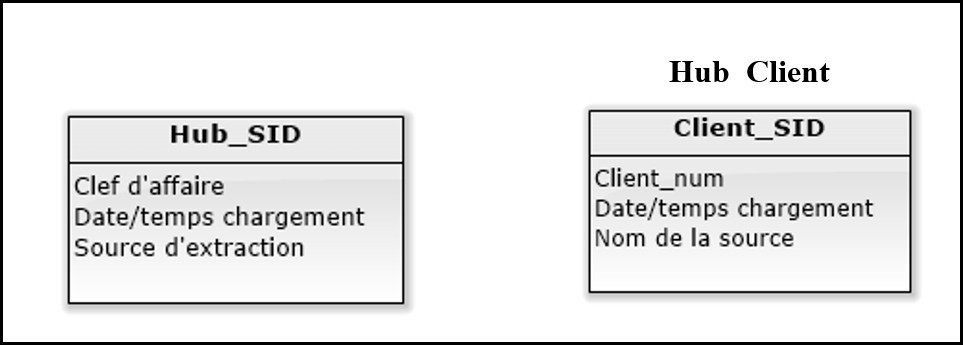
\includegraphics[width=0.7\linewidth]{./images/19}
\end{center}

\caption{Structure de l’entité hub et un exemple \citep{7}}
\label{fig:19}

\end{figure}

\textcolor{black}{La table Hub\_Client ci-avant contient :}

\begin{itemize}
\item \textbf{Client\_SID :}	 représente la clé de substitution, elle est généralement générée à partir du système de l’entrepôt de données.

\item	\textbf{Client\_num :} Un numéro qui identifie le concept d’affaire Client. 

\item	\textbf{Date/temps de chargement :} la date et le temps de la première injection de la clé dans l’entrepôt de données.


\item	\textbf{Source d’extraction :} représente le système source d’où on a pris l’information, elle est utilisée pour la traçabilité des données.

\end{itemize}


\subsubsection{Lien(Link)}
\paragraph{Définition du lien}

\textcolor{black}{Les liens sont des entités associatives. Elles lient ensemble au moins deux hubs, autrement dit, elles mettent en relation des concepts d’affaires\citep{7}.}

\textcolor{black}{Le but de l’entité lien est d’enregistrer continûment toutes les relations qui aient lieu entre les éléments de données et ceci au plus bas niveau de granularité\citep{awel2014}.
}

\textcolor{black}{La granularité d’un lien est imposée par les hubs en relation avec le lien, c’est comme dans le cas des faits d’un modèle dimensionnel où la granularité du fait est dictée par les dimensions qui rentrent en relation avec la table de fait.}

\textcolor{black}{Les liens, comme les hubs, ne contiennent pas des données descriptives, mais apparaissent dans une autre entité appelée satellite que nous expliquons après.}

\textcolor{black}{Selon les besoins d’interrogation de l’entreprise, un ensemble de métadonnées peuvent être ajoutées au lien comme les mises à jour faites, l’évaluation de confidentialité, le cryptage de la clé, etc.}

\paragraph{Structure du lien }

\textcolor{black}{La structure de l’entité lien contient les éléments nécessaires suivant\citep{awel2014} : }

\begin{itemize}

\item	\textbf{Clés de substitution des hubs :} les clés d’affaires des différents hubs et liens en relation. Elles sont obligatoires pour l’entité lien.

\item	\textbf{Clé de substitution du lien :}  Elle est optionnelle mais peut être une clé primaire obligatoire dans le cas où le lien est associé à d’autres liens.

\item	\textbf{Date de chargement :} une clé obligatoire qui enregistre quand l’association a été introduite la première fois.


\item \textbf{ Source d’extraction:}  une clé obligatoire qui référence le système source, elle est utilisée pour des fins de traçabilité et d’intégration.

\end{itemize}

\textcolor{black}{La figure suivante montre un exemple d’un lien.}

\begin{figure}[H]

\begin{center}
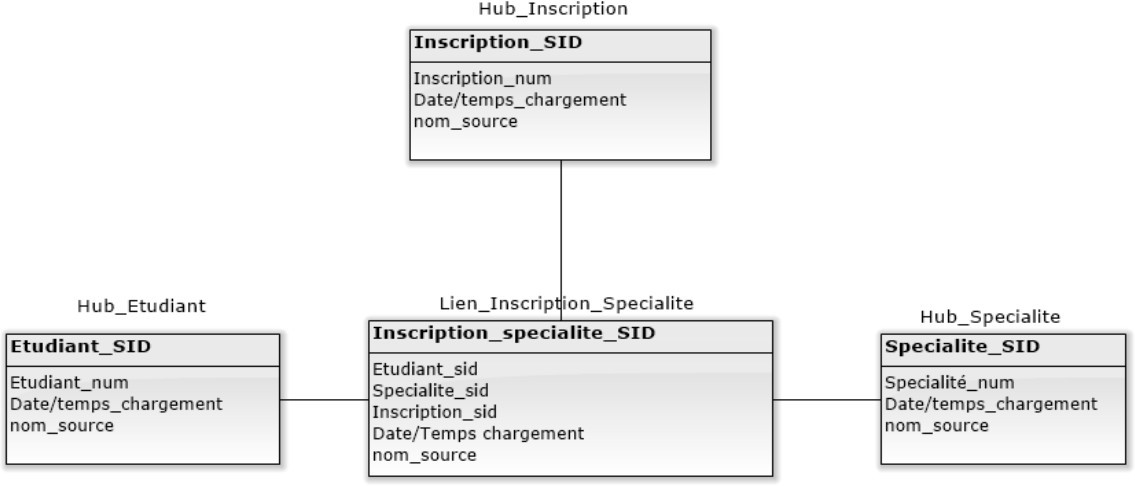
\includegraphics[width=0.8\linewidth]{./images/20}
\end{center}

\caption{Exemple d’un lien}
\label{fig:20}

\end{figure}

\subsubsection{Satellite}

\paragraph{Définition du satellite :}

\textcolor{black}{Les satellites contiennent les données qui décrivent les hubs et les liens à un moment donné et à travers le temps. Ces entités contiennent le contexte (provenant des processus d'affaires) d'un hub ou d'un lien\citep{7}.}

\textcolor{black}{Un satellite ne peut avoir qu’une seule table parent, celle qui le décrit. Par contre un hub ou un lien peuvent avoir plusieurs satellites.
Les satellites capturent les changements des données descriptives de l’entrepôt de données lorsqu’ils surviennent.}

\paragraph{Structure du satellite :}

\textcolor{black}{La structure de l’entité Satellite se compose des éléments suivants : clé de substitution du hub ou du lien qu’il décrit, date du chargement et source d’extraction. Des métadonnées peuvent être ajoutées au satellite.}

\textcolor{black}{La clé primaire du satellite est obtenue en combinant la clé du parent (hub ou lien) et la date du chargement.}

\textcolor{black}{La figure suivante montre trois exemples de satellites du hub Employé.}

\begin{figure}[H]

\begin{center}
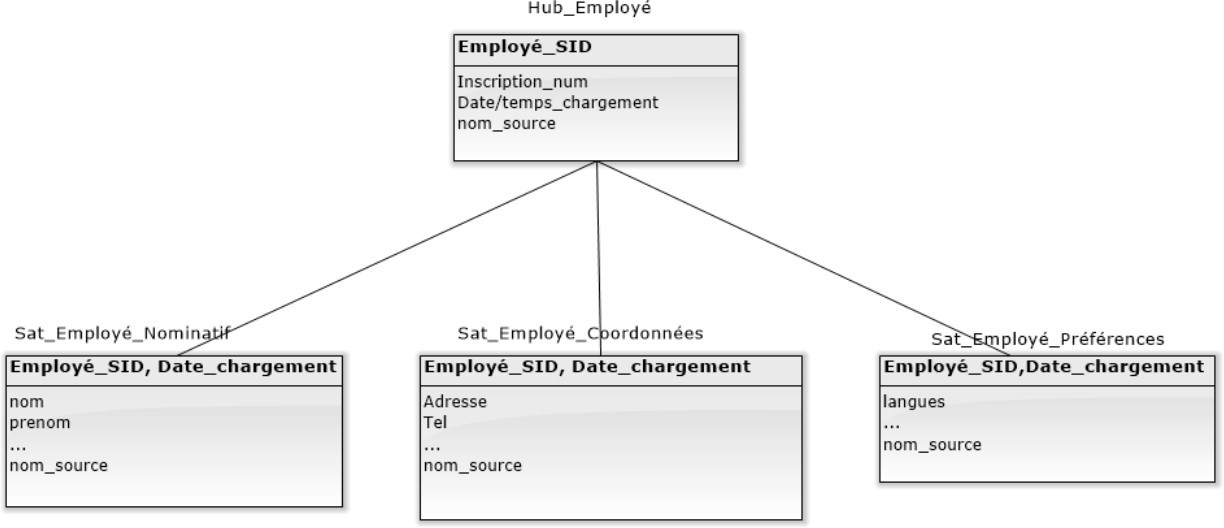
\includegraphics[width=0.8\linewidth]{./images/21}
\end{center}

\caption{Trois satellites du hub Employé}
\label{fig:21}

\end{figure}

\subsection{Architecture de l’entrepôt de données du Data Vault}

\textcolor{black}{Data Vault repose sur une architecture 3-tiers afin de séparer l’entrepôt de données brut des utilisateurs finaux et les différentes couches d’exploitation de données. Cette isolation permet de réduire les coûts engendrés par les changements qui se produisent dans les processus d’affaires.}

\textcolor{black}{Les trois tiers de l’architecture sont : \textbf{la zone de préparation de données}, \textbf{l’entrepôt de données du Data Vault} et \textbf{les magasins de données}.}


\textcolor{black}{L’architecture du Data Vault peut marcher avec l’approche d’Inmon dans le sens où le Data vault joue le rôle de l’entrepôt centralisé de l’entreprise (ou EDW en anglais pour Entreprise Data Warehouse)\citep{awel2014}. Le Data Vault fournit les données aux magasins de données qui à leur tour constituent des référentiels pour l’exploration et l’analyse de données.
}

\textcolor{black}{a figure suivante montre l’architecture Data Vault de l’entrepôt de données de l’entreprise.}

\begin{figure}[H]

\begin{center}
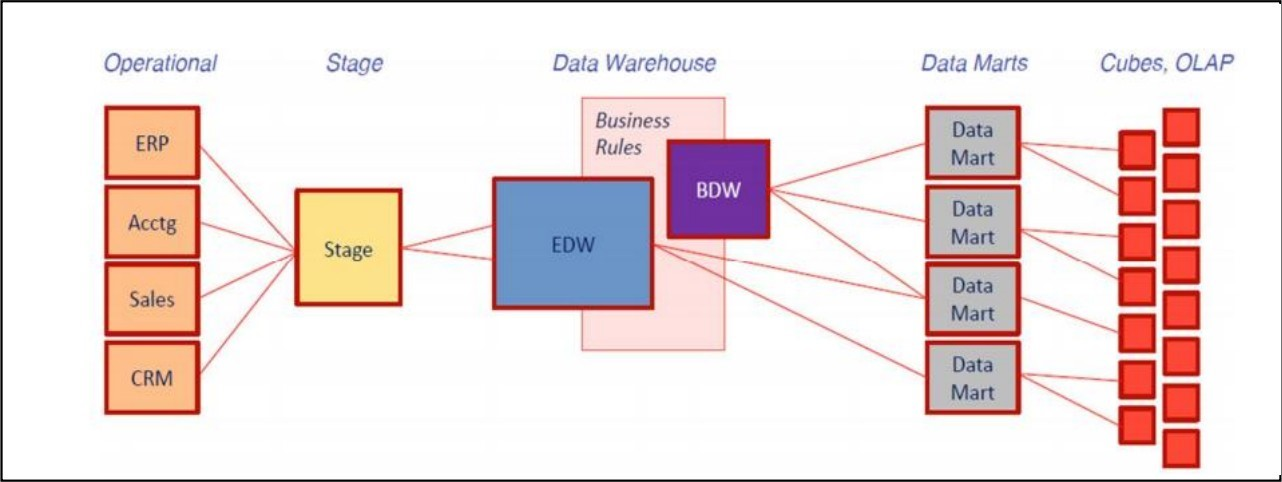
\includegraphics[width=0.9\linewidth]{./images/22}
\end{center}

\caption{Architecture de l'entrepôt Data Vault. \citep{awel2014}}
\label{fig:22}

\end{figure}


\textcolor{black}{En effet, nous constatons les couches suivantes \citep{awel2014}:}

\begin{enumerate}


\item \textcolor{black}{ \textbf{Zone de préparation:} Cette couche joue le rôle d’un batch et soutient le processus de chargement de données à partir de plusieurs sources au Data Vault. Dans cette couche, aucune règle d’affaire n’est appliquée et les données restent dans leur format d’origine. On note que les données à ce niveau ne sont pas persistantes.}

\item \textcolor{black}{ \textbf{Data Vault :}  C’est La couche noyau, elle contient les données provenant des différentes sources sans subir des transformations, c’est-à-dire les données restent brutes. Le fait de laisser les données intactes constitue une différence fondamentale des deux approches classiques.}

 \textcolor{black}{Le modèle Data Vault est composé d’un ensemble de hubs, liens et satellites qui sont les éléments principaux du modèle comme nous l’avons expliqué avant dans la partie Composants du Data Vault.}

\item \textcolor{black}{ \textbf{Entrepôt de données orienté métier (en anglais BDW pour Business Data Warehouse) :} Cette couche contient les données résultant de l’application des différentes règles métiers  comme l’alignement des données avec les clés d’affaires.}

\item \textcolor{black}{\textbf{Magasins de données :} c’est la couche de présentation, elle est déployée en utilisant une modélisation dimensionnelle. Les magasins prennent les données à partir de l’entrepôt d’affaires et du Data Vault. On note que les données à ce niveau ne sont pas persistantes. Les magasins à leur tour fournissent les données aux cubes OLAP pour les exploiter dans le Reporting, Data mining, etc.
}
\end{enumerate}


\subsection{Processus de développement du Data Vault}

\textcolor{black}{La méthodologie Data Vault se base principalement sur le modèle SEI/CMMI\footnote{http://www.tutorialspoint.com/cmmi/index.htm} 5  des meilleures pratiques et les combine avec les meilleures pratiques de Six Sigma, TQM, et SDLC. En particulier, il est axé sur une méthodologie agile pour la construction et le déploiement. 
L’équipe utilisant la méthodologie Data Vault sera automatiquement adaptée pour les projets reproductibles, cohérents et mesurables qui sont inclus dans le CMMI niveau 5}

\subsubsection{Data Vault  et SEI/CMMI }

\textcolor{black}{}
CMMI (acronyme de Capability Maturity Model Integration), est un modèle de référence, un ensemble structuré de bonnes pratiques, destiné à évaluer et mesurer la maturité du processus de développement des systèmes informatiques d’une entreprise. 

\textcolor{black}{}
Le modèle CMMI comprend cinq niveaux de maturité qui sont : initial, discipliné, ajusté, géré quantitativement et optimisé.

Chaque niveau du modèle se base sur le niveau qui le précède. Une organisation ne peut pas aboutir à un niveau sans avoir passer avec succès le niveau directement inférieur.

\textcolor{black}{Le dernier niveau sert comme une base pour l’approche Data Vault. L’organisation qui a acquis ce niveau est dans une boucle permanente d’optimisation  des processus et des technologies.}

\textcolor{black}{L’alignement du modèle de données avec les niveaux de maturité du CMMI est critique et doit inclure : la répétition, la redondance, la fiabilité et la flexibilité \citep{linstedt2009} .}

\textcolor{black}{Par exemple, le niveau quatre du CMMI inclut l’optimisation du modèle de données pour des besoins de l’entreprise. Le niveau cinq s’intéresse à l’optimisation de l’architecture du Data Vault. A ce niveau (cinq), les changements sont engagés automatiquement.}

\textcolor{black}{L’approche Data Vault met en place une gestion de projet solide. Linstedt incite l’équipe projet à faire le lien entre les composants du projet qui sont : Structure de découpage de projet,  structure de découpage organisationnel et structure de découpage de données, et établir un plan pour pouvoir suivre le projet tout le temps \citep{linstedt2009}.}

\subsubsection{Construction du Data Vault}

\textcolor{black}{Les étapes suivantes sont requises pour construire le Data Vault \citep{10} :
}

\begin{itemize}

\item	\textbf{Identification des concepts d’affaire :} cette étape consiste en l’identification des sujets d’affaires exercés par l’entreprise. Les interviews sont le cœur de cette étape.

\item	\textbf{Modéliser les hubs :} Cela nécessite une compréhension des clés d’affaires et de leur utilisation dans le cadre des concepts d’affaires identifiés.

\item	\textbf{Analyser les relations d’affaires :} cette étape consiste à identifier les relations qui lient les différents concepts d’affaire.

\item	\textbf{Modéliser les liens :} En se basant sur l’analyse des relations d’affaires, il est temps de modéliser les liens qui mettent en relation les hubs déjà modélisés. 


\item	\textbf{Modéliser les satellites :} Il s’agit de fournir un contexte aux différents hubs et liens en ajoutant des données descriptives pour chaque entité.

\end{itemize}

\textcolor{black}{On constate qu’il y a plusieurs règles qui régissent la modélisation du Data Vault. Nous énumérons une liste non exhaustive constituée de règles  suivantes\citep{3} :}

\begin{itemize}

\item	Les hubs doivent être raccordés par des liens.

\item	Les liens peuvent être raccordés à d’autres liens.

\item	Les liens doivent avoir au moins deux hubs associés avec eux afin d'être instanciés.

\item	Les clés de substitution peuvent être utilisées par les hubs et par les liens.

\item	Les clés de substitution ne peuvent pas être utilisées pour les satellites.

\item	Les clés d’affaires des hubs ne change jamais.

\item	Les satellites peuvent être connectés à un hub ou à un lien.

\item	Les liens peuvent avoir une clé de substitution.

\item	Les données sont réparties dans les structures de satellite en se basant sur le type d'information et le taux de variation.

\end{itemize}


\subsubsection{Elaboration des magasins de données}

\textcolor{black}{Dans cette phase, l’équipe projet procède à définir les besoins des décideurs par différents moyens comme les interviews et les meetings, la rédaction des décideurs d’un document qui comporte leurs besoins, etc.}

\textcolor{black}{L’équipe projet peut ensuite développer les magasins de données pour permettre aux utilisateurs d’exploiter leurs données et en tirer de l’information utile.}

\textcolor{black}{
Le développement des magasins suit la modélisation dimensionnelle de Kimball (Section II.2.5.3) vu sa rigueur en termes de performance d’interrogation.
}

\subsubsection{Chargement de données dans le Data Vault}

\textcolor{black}{Après avoir modélisé le Data Vault, on procède au chargement de données dans les structures du Data Vault (hubs, liens et satellites).}

\textcolor{black}{Le chargement d'un entrepôt de données est réalisé avec des modes de traitement différents. Souvent, les entrepôts de données sont chargés dans un mode discontinu. }

\textcolor{black}{Dans ce mode, un nombre de transactions similaires à traiter sont groupées. Ces opérations accumulées sont ensuite présentées à l'entrepôt de données à des intervalles de temps réguliers \citep{awel2014}.
}

\textcolor{black}{Une autre façon de traitement des données est le traitement en ligne. Elle implique un système à accès direct. En effet, les données entrant dans le système sont transmises directement à l'utilisateur final sous un format de sortie spécifique \citep{awel2014}.}

\subsection*{Conclusion}

\textcolor{black}{A travers ce chapitre, nous avons introduit les trois approches les plus célèbres dans le domaine de modélisation des entrepôts de données à savoir : l’approche d’Inmon, l’approche de Kimball et l’approche Data Vault.}


\textcolor{black}{L’approche d’Inmon consiste à construire un grand entrepôt de données à l’échelle de toute l’entreprise. Cet entrepôt va ensuite alimenter des magasins de données. L’approche est basée sur les modèles entité-association de l’entreprise.}


\textcolor{black}{L’approche de Kimball  consiste à construire des magasins de données indépendants un par un, puis à  les  regrouper par des niveaux intermédiaires jusqu'à obtention d'un entrepôt. Cette approche est basée sur le concept de modélisation dimensionnelle.}


\textcolor{black}{L’approche Data Vault, quant à elle, consiste à créer dans un premier temps le Data Vault qui va stocker les données brutes provenant des différentes sources. Le Data Vault se base sur la modélisation hub-lien-satellite qui sépare les données structurelles des données descriptives.}


\textcolor{black}{Le Data Vault alimente ensuite les magasins après avoir appliqué les différentes règles d’affaires. Les magasins sont déployés en utilisant la modélisation dimensionnelle.}


\textcolor{black}{Dans le chapitre suivant, nous présenterons une comparaison entre ces trois approches en s’appuyant sur différents critères.}


\chapter{Étude Comparative}
\section*{Introduction}
\addcontentsline{toc}{section}{Introduction}

\textcolor{black}{Une entreprise qui veut opter pour un système décisionnel doit réfléchir profondément sur la méthodologie à adopter pour le construire car comme tout projet, un système décisionnel mobilise des gens, génère des coûts et est plein de risques et exposé à l’échec.}
\\

\textcolor{black}{Le choix de la méthode repose, d’une part, sur la connaissance profonde de l’entreprise et ses orientations et d’autre part, sur l’analyse critique des méthodes existantes afin d’aboutir à l’approche propice.}  
\\

\textcolor{black}{Dans ce chapitre, nous effectuons, dans un premier temps, une comparaison basée sur plusieurs critéres entre les trois méthodes étudiées (Inmon, Kimball et Data Vault). Ces critéres ont été définis aprés avoir fait une étude approfondie sur les differentes approches ainsi que des discussions avec des experts Microsoft, des chefs de projets BI et des enseignants spécialisés en intégrations de données. Dans un deuxième temps, nous partageons notre vision personnelle et nous citons des recommandations qui aident à choisir la meilleure méthode dans une situation donnée.}


\section{Analyse comparative}
\textcolor{black}{\citep{breslin2004data} constate que les approches de Kimball et Inmon ressemblent du fait qu’ils utilisent des processus ETL pour alimenter l’entrepôt de données.}

\textcolor{black}{\citep{12}constate que la similarité entre l’approche Data Vault et l’approche de Kimball réside dans l’implémentation itérative de la solution et l’utilisation d’une zone de préparation pour la récupération et la synchronisation.}

\textcolor{black}{L’approche Data Vault et l’approche d’Inmon se mettent d’accord sur le fait que l’entrepôt est le plus grand référentiel de l’entreprise (EWD).}

\textcolor{black}{Malgré ces petites similarités, les différences entre les trois approches sont plusieurs et profondes.}

\textcolor{black}{Les différences importantes apparaissent dans les méthodologies de développement, la modélisation de données, l’architecture de l’entrepôt et le management du cycle de vie.}

\textcolor{black}{Ces différences sont résumées dans le tableau ci-dessous, qui est basé sur nos recherches et evaluations ainsi que les travaux de \citep{breslin2004data}, \citep{weir2008}, \citep{schneider2014com}, \citep{schalk14} et \citep{13} }
 \subsection{Méthodologie et architecture}
 \textcolor{black}{La table \ref{table31} représente une comparaison des trois approches  basée sur l'architecture de l'entrepôt, la méthodologie de développement, la complexité générale de l'approche ainsi que le coût et le temps de la mise en place de l'entrepôt de données.}


\begin{table}[H]
	\centering
	\begin{adjustbox}{center}
		\begin{tabular}{lll|l|l|l|}
			\cline{4-6}
			&                       &                                                                                      & \textbf{Relationnelle}                                                                                                                            & \textbf{Dimensionnelle}                                                                                                          & \textbf{Data Vault}                                                                                                     \\ \cline{3-6} 
			& \multicolumn{1}{l|}{} & \textbf{\begin{tabular}[c]{@{}l@{}}Structure \\ architecturale\end{tabular}}         & \begin{tabular}[c]{@{}l@{}}L’entrepôt de données \\ atomique (EDW) \\ alimente les magasins \\ de données \\ départementaux.\end{tabular}         & \begin{tabular}[c]{@{}l@{}}L’ensemble des magasins\\ de données constitue \\ l’entrepôt de l’entreprise.\end{tabular}            & \begin{tabular}[c]{@{}l@{}}Le Data Vault alimente\\ les magasins de données.\end{tabular}                               \\ \cline{3-6} 
			& \multicolumn{1}{l|}{} & \textbf{Complexité}                                                                  & Assez complexe.                                                                                                                                   & Simple.                                                                                                                          & Simple.                                                                                                                 \\ \cline{3-6} 
			& \multicolumn{1}{l|}{} & \textbf{\begin{tabular}[c]{@{}l@{}}Méthodologie \\ de \\ développement\end{tabular}} & \begin{tabular}[c]{@{}l@{}}Inspirée de la\\   méthodologie spirale.\end{tabular}                                                                  & \begin{tabular}[c]{@{}l@{}}Basée sur un processus \\ four-step (quatre étapes).\\ \end{tabular}                          & \begin{tabular}[c]{@{}l@{}}Basée sur une\\ méthodologie agile.\end{tabular}                                             \\ \cline{3-6} 
			& \multicolumn{1}{l|}{} & \textbf{\begin{tabular}[c]{@{}l@{}}Coûts de \\ déploiement\end{tabular}}             & \begin{tabular}[c]{@{}l@{}}Les coûts initiaux sont \\ plus élevés et les \\ coûts ultérieurs du\\  développement sont \\ inférieurs.\end{tabular} & \begin{tabular}[c]{@{}l@{}}Les coûts initiaux sont\\ inférieurs. Chaque phase\\ ultérieur coûte presque \\ le même.\end{tabular} & \begin{tabular}[c]{@{}l@{}}Le coût du projet est \\ inférieur par rapport \\ aux deux autres \\ approches.\end{tabular} \\ \cline{3-6} 
			& \multicolumn{1}{l|}{} & \textbf{\begin{tabular}[c]{@{}l@{}}Temps de \\ déploiement\end{tabular}}             & Longue durée.                                                                                                                                     & Courte durée.                                                                                                                    & Courte durée                                                                                                            \\ \cline{3-6} 
		\end{tabular}
\end{adjustbox}
	\caption{Comparaison entre les approches selon la Méthodologie et l'Architecture}
	\label{table31}
\end{table}	

\subsection{Modélisation de données	}
\textcolor{black}{La modélisation de données  diffère selon le modèle choisi, L'orientation ainsi que les outils utilisés lors de la modélisation. La table \ref{table32} présente une comparaison de la manière de modélisation des données selon les trois approches. Cette comparaison est basée sur les outils, l'orientation des données ainsi que l'implication de l'utilisateur final dans le processus de modélisation.}

\begin{table}[H]
	\centering
	\begin{adjustbox}{center}
		\begin{tabular}{lll|l|l|l|}
			\cline{4-6}
			&                       &                                                                                         & \textbf{Relationnelle}                                                                        & \textbf{Dimensionnelle}                                                 & \textbf{Data Vault}                                                                        \\ \cline{3-6} 
			& \multicolumn{1}{l|}{} & \textbf{\begin{tabular}[c]{@{}l@{}}Orientation de \\ données\end{tabular}}              & Pilotée par les données.                                                                      & Orientée processus.                                                     & Orientée processus.                                                                        \\ \cline{3-6} 
			& \multicolumn{1}{l|}{} & \textbf{Outils}                                                                         & \begin{tabular}[c]{@{}l@{}}Outils classiques de \\ modélisation \\ (ERDs, DISs).\end{tabular} & \begin{tabular}[c]{@{}l@{}}Modélisation\\   dimensionnelle\end{tabular} & \begin{tabular}[c]{@{}l@{}}Modélisation\\   des hubs, liens \\ et satellites.\end{tabular} \\ \cline{3-6} 
			& \multicolumn{1}{l|}{} & \textbf{\begin{tabular}[c]{@{}l@{}}Implication\\   de l’utilisateur final\end{tabular}} & Faible.                                                                                       & Forte.                                                                  & Forte.                                                                                     \\ \cline{3-6} 
		\end{tabular}
		\end{adjustbox}
	\caption{Comparaison entre les approches selon la Modélisation de données}
	\label{table32}
\end{table}	






\subsection{Philosophie}
\textcolor{black}{Chaque approche démarre d'une philosophie qui peut être proche ou totalement différentes des deux autres approches. L'acteur primaire visé par l'approche et les objectifs de chacune des trois approches sont présentés dans la table \ref{table33}. }

\begin{table}[H]
	\centering
	\begin{adjustbox}{center}
		\begin{tabular}{lll|l|l|l|}
			\cline{4-6}
			&                       &                                                                        & \textbf{Relationnelle}                                                                                                                   & \textbf{Dimensionnelle}                                                                                                                            & \textbf{Data Vault}                                                                                                                                                                                    \\ \cline{3-6} 
			& \multicolumn{1}{l|}{} & \textbf{\begin{tabular}[c]{@{}l@{}}Acteurs\\   primaires\end{tabular}} & Les professionnels d’IT.                                                                                                                 & Les utilisateurs finaux.                                                                                                                           & Les utilisateurs finaux.                                                                                                                                                                               \\ \cline{3-6} 
			& \multicolumn{1}{l|}{} & \textbf{Objectifs}                                                     & \begin{tabular}[c]{@{}l@{}}Fournir une solution technique \\ complète basée sur des \\ méthodes et technologies\\ prouvées.\end{tabular} & \begin{tabular}[c]{@{}l@{}}Fournir une solution \\ qui facilite l’interrogation\\  directe de données par \\ les utilisateurs finaux.\end{tabular} & \begin{tabular}[c]{@{}l@{}}Fournir une solution \\ technique solide et \\ complète comblant \\ les lacunes des solutions\\ classiques.\\  Elle est basée sur\\  des méthodes \\ prouvées.\end{tabular} \\ \cline{3-6} 
		\end{tabular}
	\end{adjustbox}
	\caption{Comparaison entre les approches selon la philosophie}
	\label{table33}
\end{table}	



\subsection{Intégration de données et ETL}
\textcolor{black}{Un élément clé dans le choix d’une approche est la possibilité d’une intégration simple et efficace de plusieurs sources de données. Cet élément est expliqué dans la table \ref{table34} à travers une comparaison entre la possibilité d’une intégration de sources multiples et une mesure de complexité du processus ETL.}

\begin{table}[H]
	\centering
	\begin{adjustbox}{center}
		\begin{tabular}{lll|l|l|l|}
			\cline{4-6}
			&                       &                                                                                          & \textbf{Relationnelle}                                                                                                                                                           & \textbf{Dimensionnelle}                                                                                                               & \textbf{Data Vault}                                                                                                                   \\ \cline{3-6} 
			& \multicolumn{1}{l|}{} & \textbf{\begin{tabular}[c]{@{}l@{}}Intégration\\   de sources \\ multiples\end{tabular}} & \begin{tabular}[c]{@{}l@{}}Les règles de \\ transformation doivent\\ être,implémentées\\ dans les processus ETL.\end{tabular}                                                    & \begin{tabular}[c]{@{}l@{}}Les règles de \\ transformation doivent\\ être implémentées \\ dans les processus ETL.\end{tabular}        & \begin{tabular}[c]{@{}l@{}}La séparation des satellites\\  et des clés d’affaires\\  diminue fortement la \\ complexité.\end{tabular} \\ \cline{3-6} 
			& \multicolumn{1}{l|}{} & \textbf{\begin{tabular}[c]{@{}l@{}}Complexité\\   du processus \\ ETL\end{tabular}}      & \begin{tabular}[c]{@{}l@{}}Les règles de \\ transformations sont \\ simples quand le \\ modèle de données\\ est similaire aux \\ modèles des sources\\ de données.\end{tabular} & \begin{tabular}[c]{@{}l@{}}Les transformations entre \\ les modèles OLTP et le \\ modèle dimensionnel \\ sont complexes.\end{tabular} & \begin{tabular}[c]{@{}l@{}}Les règles sont simples \\ pour charger les hubs,\\  liens et satellites.\end{tabular}                     \\ \cline{3-6} 
		\end{tabular}
	\end{adjustbox}
	\caption{Comparaison entre les approches selon l'intégration de données et ETL}
	\label{table34}
\end{table}	

\subsection{Management du cycle de vie}
\textcolor{black}{La finalité des trois approches est de concevoir et mettre en place un entrepôt de données qui réponde aux besoins et aux attentes des utilisateurs. Ceci n’est pas suffisant pour une entreprise qui a des besoins instables, flexibles et qui changent au cours du temps. D'autres critères peuvent être rajoutés tels que la facilité du changement, la traçabilité et la performance d’interrogation. La table \ref{table35} résume les critères cités précédemment.}



\begin{table}[H]
	\centering
	\begin{adjustbox}{center}
\begin{tabular}{lll|l|l|l|}
	\cline{4-6}
	&                       &                                                                                                                             & \textbf{Relationnelle}                                                                                                                                                                                           & \textbf{Dimensionnelle}                                                                                                                                                                  & \textbf{Data Vault}                                                                                                                                                                                                         \\ \cline{3-6} 
	& \multicolumn{1}{l|}{} & \textbf{\begin{tabular}[c]{@{}l@{}}Flexibilité\\ contre le \\ changement \\ du modèle \\ de données\\ sources\end{tabular}} & \begin{tabular}[c]{@{}l@{}}Nécessité de \\ changements\\ dans les tables.\end{tabular}                                                                                                                           & \begin{tabular}[c]{@{}l@{}}Souvent les \\ changements \\ du modèle \\ source influent\\ sur le modèle de \\ données de l’entrepôt.\end{tabular}                                          & \begin{tabular}[c]{@{}l@{}}Les tables existantes \\ ne sont pas affectées.\\ Le seul changement\\ est l’ajout des satellites\\ appropriés.\end{tabular}                                                                     \\ \cline{3-6} 
	& \multicolumn{1}{l|}{} & \textbf{\begin{tabular}[c]{@{}l@{}}Flexibilité\\ contre les \\ nouveaux \\ besoins \\ d’analyse\end{tabular}}               & \begin{tabular}[c]{@{}l@{}}Le modèle change \\ seulement si les \\ données  exigées \\ n’existent pas \\ dans l’entrepôt.\end{tabular}                                                                           & \begin{tabular}[c]{@{}l@{}}Les nouveaux \\ besoins ont un \\ impact sur le \\ modèle de \\ données.\end{tabular}                                                                         & \begin{tabular}[c]{@{}l@{}}Aucun changement ne \\ sera fait sur le modèle\\ du Data Vault. \\ Seulement \\ la livraison de données \\ aux magasins qui doit\\ être adaptée.\end{tabular}                                    \\ \cline{3-6} 
	& \multicolumn{1}{l|}{} & \textbf{\begin{tabular}[c]{@{}l@{}}Facilité de\\ changement\\ du modèle\end{tabular}}                                       & \begin{tabular}[c]{@{}l@{}}Les données \\ historiques doivent\\ être migrées \\ dans certains cas.\end{tabular}                                                                                                  & \begin{tabular}[c]{@{}l@{}}Le refactoring de \\ certaines tables \\ est nécessaire dans \\ certains cas.\end{tabular}                                                                    & \begin{tabular}[c]{@{}l@{}}Les tables existantes \\ ne sont pas affectées.\\ Le seul changement \\ est l’ajout des\\   satellites appropriés.\end{tabular}                                                                  \\ \cline{3-6} 
	& \multicolumn{1}{l|}{} & \textbf{\begin{tabular}[c]{@{}l@{}}Audit et\\ traçabilité\end{tabular}}                                                     & \begin{tabular}[c]{@{}l@{}}L’information \\ historique est \\ capturée en insérant\\ un nouvel \\ enregistrement à \\ chaque fois les \\ données sources\\ changent.\end{tabular}                                & \begin{tabular}[c]{@{}l@{}}Utilise le concept \\ de « Dimension à \\ évolution lente\footnote{On parle d'une dimension à évolution lente lorsqu'une dimension peut subir des changements de description des attributs.}{}{} »\\ pour enregistrer le\\ changement \\ d’historique.\end{tabular}                           & \begin{tabular}[c]{@{}l@{}}L’information historique\\ est capturée en insérant\\ des nouveaux liens et\\ satellites.\end{tabular}                                                                                           \\ \cline{3-6} 
	& \multicolumn{1}{l|}{} & \textbf{\begin{tabular}[c]{@{}l@{}}Performances\\   d’interrogation\end{tabular}}                                           & \begin{tabular}[c]{@{}l@{}}L’interrogation est \\ très lente à cause \\ de la structure 3NF \\ de données.\\ Les magasins \\ dimensionnels\\ sont nécessaires \\ pour l’analyse et \\ le reporting.\end{tabular} & \begin{tabular}[c]{@{}l@{}}Le modèle est conçu\\ pour être très \\ performant en \\ interrogation en \\ dénormalisant les\\   dimensions et \\ laissant les faits\\ en 3NF.\end{tabular} & \begin{tabular}[c]{@{}l@{}}L’interrogation directe\\ est très lente à cause \\ de la haute normalisation\\ de données. \\ Les magasins dimensionnels \\ sont nécessaires \\ pour l’analyse et \\ le reporting.\end{tabular} \\ \cline{3-6} 
\end{tabular}
	\end{adjustbox}
	\caption{Comparaison entre les approches selon le management du cycle de vie}
	\label{table35}
\end{table}






\section{Appréciation personnelle}
\textcolor{black}{Comme la matrice de comparaison précédente le montre, aucune approche ne répond parfaitement à tous les critères. Chaque méthode a ses avantages et ses inconvénients.}

\textcolor{black}{Dans ce qui suit et à travers l’étude comparative des trois approches que nous avons effectuée, nous proposons quelques recommandations qui permettent de répondre à la question « Quelle approche dans quelle situation ? ».} 
\\
\begin{itemize}
	\item  \begin{bf}Approche d’Inmon : \end{bf}cette approche est recommandée quand les besoins d’analyse ne sont pas définis ou le but de l’entrepôt est de fournir les informations à plusieurs systèmes BI. Elle est aussi préférée si les structures du système source sont relativement stables.
	\item  \begin{bf}Approche de Kimball : \end{bf}cette approche est fortement recommandée pour les magasins de données vu que le modèle dimensionnel offre une haute performance d’interrogation et il est compréhensible par les utilisateurs finaux. En outre, elle est aussi appropriée pour développer l’entrepôt si les besoins sont connus et bien définis.
	\item  \begin{bf}Approche Data Vault : \end{bf}c’est une approche puissante pour développer l’entrepôt  quand il y a plusieurs sources de données avec des changements réguliers des structures de ces sources. Elle est efficace dans les environnements de projets agiles. Si la flexibilité, la productivité et l’évolutivité de l’entrepôt sont les préoccupations de l’entreprise alors l’adoption du Data Vault est le meilleur choix.
\end{itemize}


\section*{Conclusion}
\addcontentsline{toc}{section}{Conclusion}
\textcolor{black}{A l’issue de ce chapitre, nous avons vu les similarités et les différences entre les trois approches en nous s’appuyant sur certains critères dont les plus importants  sont la méthodologie de développement, l’architecture et la modélisation de données.}  

\textcolor{black}{Nous avons constaté aussi qu’il n’y a pas une approche parfaite, mais avec la connaissance de la situation de l’entreprise nous pouvons opter pour l’une ou l’autre.}\\


\newpage 


\chapter{Cas pratique}
\section{Présentation de l’organisme d’accueil }
\textcolor{black}{ExterionMedia capitalise plus de 100 ans d’expérience en Communication Extérieure notamment au travers de sa marque locale emblématique Giraudy \citep{Exterion}.}

\textcolor{black}{Son activité principale consiste à commercialiser des espaces publicitaires en France dans toutes les agglomérations de plus de 20 000 habitants au plus près des consommateurs. Ils créent la différence avec un patrimoine de qualité dont la diversité d’environnements, la variété d’implantation et des formats, offrent des solutions sur mesure, puissantes et adaptées aux besoins des annonceurs \citep{Exterion}.}

\textcolor{black}{Grâce à leurs dispositifs Grand Format, leurs mobiliers urbains, leurs toiles évènementielles, leurs écrins, et leurs écrans digitaux, ils mobilisent l’audience de la rue autour des marques \citep{Exterion}.}


\begin{figure}[H]

\begin{center}
\includegraphics[width=0.9\linewidth]{./images/30}
\end{center}

\caption{Quelques chiffres sur ExterionMedia \citep{Exterion}}
\label{fig:1}

\end{figure}

\begin{figure}[H]

\begin{center}
\includegraphics[width=0.9\linewidth]{./images/31}
\end{center}

\caption{Changement de ExterionMedia \citep{Exterion}}
\label{fig:1}

\end{figure}


\section{Etudes des besoins }
\textcolor{black}{Tout Data Warehouse doit être en mesure de répondre aux attentes des utilisateurs.
Cela ne peut, évidemment, se faire sans une étude approfondie de leurs besoins. }

\textcolor{black}{Durant l’étude des besoins on ne peut se limiter aux interviews avec les utilisateurs, néanmoins, il faudrait absolument prendre en compte l’avis des administrateurs des bases de données des systèmes sources : « les DBA sont les principaux experts sur les applications existantes susceptibles d'alimenter l'entrepôt de données. Leurs interviews servent à confronter aux réalités certains des thèmes qui surgissent lors des rencontres avec les utilisateurs finaux. » \citep{kimball1996data}.}

\begin{figure}[H]

\begin{center}
\includegraphics[width=0.7\linewidth]{./images/23}
\end{center}

\caption{La place de l’étape d’étude des besoins dans un projet Data Warehouse.}
\label{fig:1}

\end{figure}

\textcolor{black}{En effet, c'est à partir de cette étude que se décidera la manière de construction de l’entrepôt de données et de son architecture. }

\textcolor{black}{Cette étude des besoins s’est déroulée sur 5 entretiens et a concerné 4 personnes occupant différents postes à des niveaux hiérarchiques différents. L’ensemble des entretiens nous a permis tout d’abord d’appliquer les méthodes d’analyse et de collecte d’information. Il nous a aussi permis de connaître davantage de détails sur les rouages de l’entreprise et d’identifier les besoins analytiques de l’entreprise.}

\textcolor{black}{Ci-dessous une Synthétisation des besoins recensés : }


\begin{figure}[H]

\begin{center}
\includegraphics[width=1\linewidth]{./images/24}
\end{center}

\caption{Synthétisation des besoins recensés.}
\label{fig:1}

\end{figure}

\textcolor{black}{Après l’étude des besoins de l’entreprise et aussi selon l’étude comparative des trois architectures que nous avons faite, nous avons trouvé que celle de Kimball était plus optimale.}

~\

\textbf{Pourquoi Kimball ?}

~\

\textcolor{black}{L'approche Kimball est généralement la moins complexe, la plus simple et la plus rapide à mettre en œuvre, elle offre la meilleure combinaison de performances, de chargement et d'interrogation.}

\textcolor{black}{Elle est idéalement structurée pour soutenir le développement agile itératif et serait l'approche optimale pour notre entreprise et surtout que les besoins sont connus et bien définis.}



\section{Conception et mise en place de l’architecture }
\subsection{La conception d’un modèle dimensionnel  }
\textcolor{black}{La conception d’un modèle dimensionnel passe par cinq étapes essentielles :}

\begin{itemize}

	\item  \begin{bf}Choix de l’activité à modéliser : \end{bf} ce choix se fait après classement des activités dans une matrice dite d’analyse des priorités \citep{kimball2004data}. Cette matrice permet de connaître quelle activité choisir en premier. Le classement des sujets recensés s’est fait en collaboration avec les décideurs et les techniciens de l’entreprise.
	\item  Définition de l’activité et de son gain,
	\item  Définition des dimensions qui décrivent une ligne de la table de fait,
	\item  Définir les mesurable du fait,
	\item  Définir les agrégats.
\end{itemize}

\textcolor{black}{Ci-dessous un exemple sur un modèle en étoile de l’une des activités :}

\begin{figure}[H]

\begin{center}
\includegraphics[width=1\linewidth]{./images/25}
\end{center}

\caption{Modèle en étoile de l’activité « Vente ».}
\label{fig:1}

\end{figure}

\subsection{Conception de la zone « alimentation »}
\textcolor{black}{La conception du processus d’alimentation nécessite les étapes suivantes :}
~\

\begin{itemize}

	\item \begin{bf} Définition de l’activité et de son gain,
	\item  Définir les mesurable du fait,
	\item  Définir les agrégats.\end{bf}
    	\begin{itemize}
        	\item  Définition de l’activité et de son gain,
        	\item  Définir les mesurable du fait,
        	\item  Définir les agrégats.
        \end{itemize}
\end{itemize}


\textcolor{black}{Ci-dessous un diagramme d’activités qui décrit le processus général de l’alimentation de l’entrepôt de données dés sa mise en service :}

\begin{figure}[H]

\begin{center}
\includegraphics[width=1\linewidth]{./images/26}
\end{center}

\caption{Diagramme d’activité du processus d’alimentation.}
\label{fig:1}

\end{figure}

\section{Réalisation et déploiement }
\textcolor{black}{Pour la réalisation et la mise en place de la solution, il a été nécessaire de recourir à un certain nombre d’outils et mettre en place des environnements d’exécution.}

\textcolor{black}{Ci-dessous les principaux outils : }


\begin{itemize}

	\item \begin{bf} Outils d’integration de données (ETL) :\end{bf} Informatica PowerCenter
	\item \begin{bf} Matériel :\end{bf} les systemes sources sont installés sur differents plateforme :
	\begin{itemize}
        	\item Machine IBM,
        	\item Machine INTEL : HP ou DELL.
        \end{itemize}
	\item \begin{bf} système de gestion de base de données (SGBD) : \end{bf} SQL Server 
	\item \begin{bf} Outils de reporting : \end{bf} SQL Server Reporting Services ( SSRS )
    	
\end{itemize}


\section{Résultats et évaluations }
\subsection{Utilisation du stockage }
\textcolor{black}{Les données sont stockées dans un format d’utilisation finale optimisé pour les rapports.}

~\

\textbf{Pourquoi pas Inmon ou DataVault ? }

~\

\textcolor{black}{Les structures des approches Inmon et DataVault ne sont pas optimisées pour les requêtes directes et nécessitent des tableaux de données dimensionnels pour la création de rapports. Ces points de données doivent être conservés (physiques) pour tous les volumes de données, sauf les plus petits, pour des raisons de performances. Cela double essentiellement les exigences de stockage par rapport à l'approche Kimball et coutera plus à l’entreprise par la suite.}

\subsection{Complexité ETL }
\textcolor{black}{Concernant la complexité ETL, il nous a fallu un seul processus ETL unique qui charge le modèle de données final contrairement aux 2 autres approches qui nécessitent 2 processus ETL : le premier pour le chargement depuis les systèmes sources et l’autre pour la création de rapports de données.}

\textcolor{black}{Ci-dessous un exemple sur un processus ETL :}


\begin{figure}[H]

\begin{center}
\includegraphics[width=1\linewidth]{./images/27}
\end{center}

\caption{Processus ETL de la table « Agence»}
\label{fig:1}

\end{figure}

\subsection{Évolutivité ETL et performances de chargement  }
\textcolor{black}{La mise en place de l'architecture de Kimball nous a permis de prendre en charge le chargement de plusieurs domaines en parallèle (dimensions d'abord, puis faits). }


\subsection{Audit, traçabilité et conformité   }
\textcolor{black}{Utilise le concept de dimensions qui changent lentement pour suivre les changements historiques. L’ajout de nouveaux attributs est possible mais ne permet pas de recréer des modifications historiques.}

\textcolor{black}{Nous considérons ce point comme point faible si nous faisons une comparaison avec les 2 autres approches.}

\subsection{La modélisation  }
\textcolor{black}{Ce point fait partie des raisons principales pour lesquelles nous avons choisi cette approche car,  selon cette dernière, la complexité de la modélisation varie selon l'industrie ou le domaine. Une méthodologie bien établie existe avec des lignes directrices et des cadres de modélisation pour chaque type de domaine, par industrie. }

\textcolor{black}{ Puisque le modèle lui-même est exposé pour l’utilisation finale, il n'a pas besoin de modélisation supplémentaire pour capturer les données sources comme dans l'approche Inmon et Data Vault.}

\subsection{Performances de requête }
\textcolor{black}{Cette approche est conçue pour optimiser les performances des requêtes en dénormalisant les dimensions contenant des attributs et des hiérarchies de filtres et en conservant les données factuelles dans 3NF pour optimiser les performances et le stockage. Les grandes tables de faits peuvent être facilement partitionnées (généralement sur une clé de date) et indexées pour prendre en charge de hautes performances. Les technologies d'indexation en mémoire les plus récentes de column-store fonctionnent très bien pour les tables de faits et donc résultat d’exécution plus rapide par rapport aux deux autres approches qui sont trop lentes en raison de la structure hautement normalisée des données.}

\textcolor{black}{Ci-dessous un exmeple sur deux exécutions d'une méme requéte avant et aprés la mise en place de l'architecture :}



\begin{figure}[H]

\begin{center}
\includegraphics[width=1\linewidth]{./images/28}
\end{center}

\caption{Résultat d'exécution - Avant -}
\label{fig:1}

\end{figure}


\begin{figure}[H]

\begin{center}
\includegraphics[width=1\linewidth]{./images/29}
\end{center}

\caption{Résultat d'exécution  - Aprés -}
\label{fig:1}

\end{figure}






\newpage
\chapter*{Conclusion générale}
\markboth{Conclusion générale}{}
\addcontentsline{toc}{chapter}{Conclusion générale}


\textcolor{black}{La rude concurrence entre les entreprises nécessite de plus en plus la mise en place des systèmes décisionnels. Ces derniers permettent aux décideurs de prendre des décisions et des choix dans des temps très courts et ce pour un volume d’informations toujours plus important. }


\textcolor{black}{A travers ce travail de Master, nous avons vu que les systèmes décisionnels reposent sur un référentiel de stockage centralisé appelé entrepôt de données. Son rôle est d'intégrer et de stocker l'information utile aux décideurs et de conserver l'historique des données pour supporter les analyses effectuées lors de la prise de décision. }


\textcolor{black}{Les approches de modélisation des entrepôts de données sont plusieurs et diverses. Cependant, nous avons constaté que trois approches monopolisent le marché des entrepôts. Il s’agit de l’approche de Kimball, l’approche d’Inmon et l’approche Data Vault. }


\textcolor{black}{L’approche d’Inmon consiste à construire un grand entrepôt de données à l’échelle de toute l’entreprise. Cet entrepôt va ensuite alimenter des magasins de données. La modélisation de données est basée sur les modèles entité-association de l’entreprise sur lesquels on fait une série de transformations pour aboutir au modèle de données de l’entrepôt de données. }



\textcolor{black}{  Inmon n’implique pas les utilisateurs finaux dans la construction de l’entrepôt, par contre des équipes de professionnels IT sont exigées. }

\textcolor{black}{
La vision de Kimball est différente. En effet, il voit qu’un entrepôt de données n’est qu’un ensemble de magasins de données indépendants et on n’a pas besoin d’une séparation physique entre les deux. Cette approche est basée sur les concepts de la modélisation dimensionnelle où on implique fortement l’utilisateur final et l’on incite à exprimer ses besoins, ensuite on tire les faits et dimensions correspondants tout en respectant un schéma de modélisation selon les besoins de l’entreprise.}




\textcolor{black}{L’approche Data Vault, quant à elle, consiste à créer dans un premier temps le Data Vault qui va stocker les données brutes provenant des différentes sources. Le Data Vault se base sur la modélisation hub-lien-satellite qui sépare les données structurelles des données descriptives. }



\textcolor{black}{Le Data Vault alimente ensuite les magasins après avoir appliqué les différentes règles d’affaires. Les magasins sont déployés en utilisant la modélisation dimensionnelle. }



\textcolor{black}{ Nous avons aussi élaboré aussi une analyse comparative entre les trois méthodes et nous avons constaté qu’aucune approche n’est meilleure. En effet, avec la connaissance de la situation de l’entreprise et de ses orientations, nous pouvons choisir une approche plutôt qu’une autre.}


\textcolor{black}{L’approche de Kimball est préférée pour modéliser les magasins de données, vu la performance d’interrogation qu’elle fournit, particulièrement quand les besoins sont stables et bien définis contrairement à l’approche d’Inmon qui est recommandée quand les besoins ne sont pas définis ou ils sont très évolutifs. }


\textcolor{black}{Les deux approches font face à beaucoup de problèmes surtout quand les sources de données changent souvent. Cela implique un re-engineering de l’entrepôt.
Pour pallier ces problèmes, l’approche Data Vault est préconisée. Elle permet une flexibilité et une évolutivité extrêmes. Elle est recommandée quand les sources changent souvent de structures. }

\textcolor{black}{
Ensuite, nous avons présenté et comparé les approches de modélisation des entrepôts de données les plus répandues dans la littérature. Pour ce faire, nous nous sommes basés sur des travaux traitant ce sujet.}

\textcolor{black}{Au final, et après avoir établi une etude des besoins et connu la situation de notre entreprise, nous avons pu determiner l'approche la plus optimale et nous l'avons mis en place, ce qui nous a permis de vérifier de manière pratique les résultats. Mais nous envisageons, dans nos travaux futurs, d'aller plus loin et de faire des tests plus approfondis pour une évaluation plus efficace.
}
%%%%%%%%%%%%%%%%%%%%%%%%%%%%%%%%%%%%%%%%%%%%%%%%%%%%%%%%%%%%%%%%%%%%


\renewcommand{\bibname}{Bibliographie}
\fancyhead[LE,RO]{} \fancyhead[LO]{}\fancyhead[RE]{}
\renewcommand{\footrulewidth}{0.5pt}
\bibliographystyle{abbrv}
\bibliography{biblio}

\end{document}


